\documentclass[12pt,fleqn]{book} %taille de la police par défaut, et équations jusitifées à gauche
\usepackage[top=3cm,bottom=3cm,left=3.2cm,right=3.2cm,headsep=10pt,a4paper]{geometry} % marges
\usepackage{xcolor}
\definecolor{enstabGreen}{HTML}{C8D200} 	%vert  	#c8d200 
\definecolor{enstabLightGreen}{HTML}{E9ED99} 	%vert  	#c8d200 
\definecolor{enstabLightBlue}{HTML}{009EE0} %bleu clair 	#009ee0
\definecolor{enstabVeryLightBlue}{HTML}{99D8F3} %bleu clair 	#009ee0
\definecolor{enstabDarkBlue}{HTML}{005C8F}	%bleu foncé 	#005c8f
\definecolor{enstabDarkGrey}{HTML}{333333}	%gris fort 	#333333
\definecolor{enstabLightGrey}{RGB}{48,48,48}	%gris fort 	#333333
\definecolor{enstabParme}{HTML}{8878B2}		%parme 	#8878b2
\definecolor{enstabOrange}{HTML}{F18E00} 	%orange 	#f18e00
\usepackage[colorlinks=true,
        urlcolor=enstabLightBlue,
        anchorcolor=enstabDarkBlue,
        linkcolor=enstabDarkBlue,
        citecolor=enstabDarkGrey,
        pdfauthor={Johan B. C. Engelen},
        pdfkeywords={SVG; LaTeX; Inkscape},
        pdftitle={How to include an SVG image in LaTeX},
        pdfsubject={Describes how to include an SVG image easily in LaTeX using Inkscape}] {hyperref}
\usepackage{url}
\usepackage[utf8]{inputenc} % lettres accentuées
\usepackage[T1]{fontenc}    % Use 8-bit encoding that has 256 glyphs
\usepackage[frenchb]{babel} % Pour le français
\usepackage{cclicenses}     % Licences CC
\usepackage{epigraph}
\usepackage{eso-pic}        % pour une image en fond, page de titre
\usepackage{graphicx}       % Pour inclure des images
\graphicspath{{images/}}    % Où sont les images ?

\usepackage{listings}      % Pour coloriser les codes que vous insérez
\lstset{ %
  backgroundcolor=\color{white},   % choose the background color; you must add \usepackage{color} or 
  basicstyle=\footnotesize\ttfamily,        % the size of the fonts that are used for the code
  breakatwhitespace=false,         % sets if automatic breaks should only happen at whitespace
  breaklines=true,                 % sets automatic line breaking
  captionpos=b,                    % sets the caption-position to bottom
  commentstyle=\color{enstabOrange},    % comment style
  deletekeywords={...},            % if you want to delete keywords from the given language
  escapeinside={\%*}{*)},          % if you want to add LaTeX within your code
  extendedchars=true,              % lets you use non-ASCII characters; for 8-bits encodings only, does not work with UTF-8
  %frame=single,                    % adds a frame around the code
  keepspaces=true,                 % keeps spaces in text, useful for keeping indentation of code (possibly needs columns=flexible)
  keywordstyle=\color{enstabDarkBlue},       % keyword style
  %language=Octave,                 % the language of the code
  morekeywords={*,...},            % if you want to add more keywords to the set
  numbers=left,                    % where to put the line-numbers; possible values are (none, left, right)
  numbersep=8pt,                   % how far the line-numbers are from the code
  numberstyle=\tiny\color{enstabDarkGrey}, % the style that is used for the line-numbers
  rulecolor=\color{black},         % if not set, the frame-color may be changed on line-breaks within not-black text (e.g. comments (green here))
  showspaces=false,                % show spaces everywhere adding particular underscores; it overrides 'showstringspaces'
  showstringspaces=false,          % underline spaces within strings only
  showtabs=false,                  % show tabs within strings adding particular underscores
  stepnumber=5,                    % the step between two line-numbers. If it's 1, each line will be numbered
  stringstyle=\color{enstabParme},     % string literal style
  tabsize=2,                       % sets default tabsize to 2 spaces
  title=\lstname                   % show the filename of files included with \lstinputlisting; also try caption instead of title
}
\usepackage{subcaption}




\usepackage{booktabs}       % pour de jolis tableaux
%\usepackage{fancyhdr}       % pour des entêtes et pieds de pages améliorés.
\usepackage{makeidx}        % requis pour faire les index
\usepackage{glossaries} %requis pour faire le glossaire
     % Ce fichier contient tous les packages nécessaires à la compilation
\makeindex           % donne l'ordre de créer l'index
%\includegraphics[scale=1]{image}
\newacronym{IS}{IS}{Ingénierie Système}
\newacronym{WBS}{WBS}{Work Breakdown Structure}					 % contient les entrées du glossaire
\makeglossaries      % donne l'ordre de créer le glossaire

\begin{document}
\renewcommand{\contentsname}{Sommaire}                % des jolis noms pour la table des matières
%\renewcommand{\bibname}{Références bibliographiques}  % des jolis noms pour les sections bibliographiques
\renewcommand{\glossaryname}{Glossaire}               % et glossaire


%----------------------------------------------------------------------------------------
%	 PAGE DE TITRE
%-----------------------------	-----------------------------------------------------------

\begingroup
\thispagestyle{empty}
\AddToShipoutPicture*{\put(6,5){
\includegraphics[scale=1]{FondTitreSPID}}} % Image background
\begin{center}
\vspace*{2cm}
{\Huge \textsc{\textbf{Rapport d'avancement}}}\\
\vspace*{2cm}
{\Huge \textbf{BMONS}}\par % ACRONYME du projet
\vspace*{2cm}
{\huge Beehive Monitoring System}\par % Intitulé du projet
\end{center}
\vspace*{4cm}

\textbf{\huge Rédigé par :} 

\begin{center}
{
\huge
Alice Danckaers\\
Benoît Raymond\\
Etiene Dalcol\\
Nicolas Van-Nhân Nguyen\\
Tao Zheng\\
Armand Sellier\\
}
\end{center}

\vspace*{1cm}

{\huge \textbf{Sous la direction de :}}\\
\begin{center}
{\huge
Olivier Reynet\\
}
\end{center}
\endgroup


%----------------------------------------------------------------------------------------
%	COPYRIGHT PAGE
%----------------------------------------------------------------------------------------
\newpage
~\vfill
\thispagestyle{empty}

\noindent \bysa 2014 Alice Danckaers, Benoît Raymond, Etiene Dalcol, Nicolas Van-Nhân Nguyen, Tao Zheng and Armand Sellier.\\\\ % Copyright notice

%\noindent \textsc{Published by Publisher}\\ % Publisher

%\noindent \textsc{book-website.com}\\ % URL

\noindent Licensed under the Creative Commons Attribution-ShareAlike 4.0 International Public License.\\ % License information

\noindent \textit{Première impression, décembre 2014} % Printing/edition date

%----------------------------------------------------------------------------------------
%	SOMMAIRE
%----------------------------------------------------------------------------------------
\tableofcontents  % Imprime le sommaire
\cleardoublepage  % pour commencer sur une page impaire

%----------------------------------------------------------------------------------------
%	Préambules
%----------------------------------------------------------------------------------------
\frontmatter      % La partie non numérotée préalable au document principal


\chapter{Remerciements}
\epigraph{La gratitude est non seulement la plus grande des vertus, mais c'est également la mère de tous les autres.}{Emil Cioran}

L'équipe du projet BMONS (BeeHive Monitoring System) souhaiterait remercier monsieur O.Reynet, responsable de l'UV 3.4 et auteur de notre sujet ainsi que notre encadrant IS, monsieur B.CLEMENT pour leurs conseils, leur soutient et leur disponibilité. Ils ont su nous guider tout au long du projet notamment sur le plan technique et architectural de notre système. \\

Nous tenons également à remercier monsieur F.Singhoff, professeur à l'université de Bretagne Occidentale à Brest dans le domaine des systèmes embarqués et apiculteur, qui a accepté de prendre part à notre projet en tant que "client" en partageant ainsi son expérience de l'apiculture. Il a aussi mis à notre disposition une de ses ruches afin que nous puissions nous rendre compte des dimensions et de l'espace disponible pour installer notre système.
       
 

\chapter{Préambule}
\epigraph{Le chemin est long du projet à la chose.}{Molière}

\section{Comment compiler ce document ?}

Un document \LaTeX peut se compiler au travers d'un IDE (TexSutdio, TeXMaker par exemple).
Le répertoire de ce document contient également un Makefile qui permet de compiler simplement en ligne de commande. 
La fabrication du glossaire et de l'index est prise en charge par ce Makefile.
Pour l'utiliser, il suffit d'ouvrir un terminal, de se placer dans le répertoire du document puis d'invoquer la commande \texttt{make}. 


Voici les différentes cibles disponibles pour ce Makefile :
\begin{verbatim}
make                - contruit le document
make all            - contruit le document
make index          - contruit l'index
make glossaire      - contruit le glossaire
make bib            - contruit la bibliographie
make pdf            - contruit le document PDF
make clean          - supprime les fichiers LaTeX intermédiaires
make clean-all      - supprime tous les fichiers générés par la compilation
make help           - cette information
\end{verbatim}


\section{Références internes}

Les références internes sont des renvois vers des figures, des tableaux ou des sections du rapport.
\LaTeX introduit un mécanisme simple pour établir ce genre de référence, via les commandes \texttt{\textbackslash label} et \texttt{\textbackslash ref}. 
La première sert à définir une ancre dans le document, la seconde à la citer.
Voici par exemple une référence interne vers la section intitulée \textit{Approche Top-Down} (cf. section  \ref{sec:top-down}). Ce renvoi est le résultat de la commande \texttt{\textbackslash ref\{sec:top-down\}}. Si vous vous rendez dans le corps de cette section, vous y trouverez le label en question \texttt{\textbackslash label\{sec:top-down\}}. 

\subsection{Tableaux et figures}
Les figures  et les tableaux  sont référencés de la même la manière (cf. figure \ref{fig:gomboc} et tableau \ref{tab:exemple}). \index{Table} \index{Figure}

\begin{table}[h]
\centering
\begin{tabular}{lll}
\toprule
\textbf{Algorithmes} & \textbf{Performance (s)} & \textbf{Gain (dB)}\\
\midrule
Algorithme 1 & 0.0003262 & 0.562 \\
Algorithme 2 & 0.0015681 & 0.910 \\
Algorithme 3 & 0.0009271 & 0.296 \\
\bottomrule
\end{tabular}
\caption{\label{tab:exemple}Performances et gains des algorithmes envisagés.}
\end{table}

\begin{figure}[h]
\centering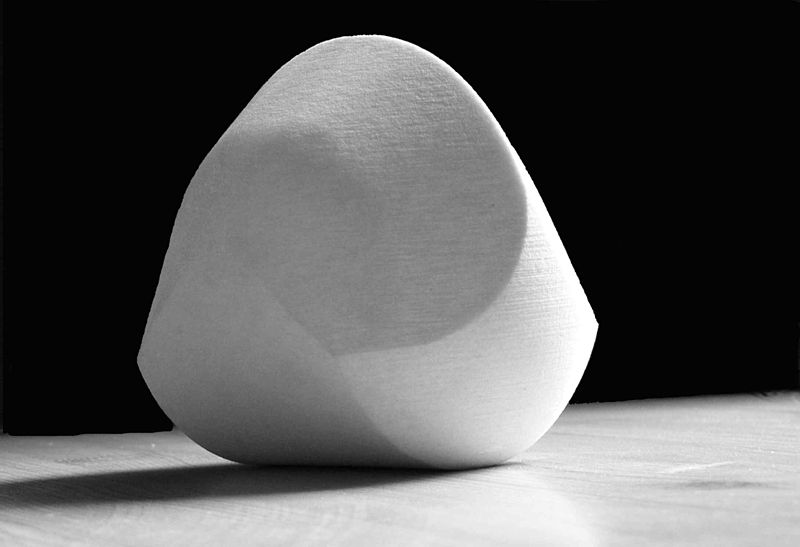
\includegraphics[scale=0.15]{Gomboc.jpg}
\caption{\label{fig:gomboc}Gömböc : un objet homogène tridimensionnel mono-monostatique. (source : Wikipedia)}
\end{figure}



\subsection{Codes}
Si vous souhaitez insérer du code dans votre rapport, invoquez les commandes : \\
 \texttt{\textbackslash lstset\{language=python\}}\\
 \texttt{\textbackslash lstinputlisting[caption=\{Titre du listing\}, label=\{lst:code\}]\{./code/code.py\}}


La première commande sélectionne le langage, pour que les mots clés de celui-ci soient correctement détectés et mis en valeur. 
La seconde commande permet d'insérer le code contenu dans le fichier code.py qui se trouve dans le sous-répertoire code.
Pour faire référence au code, il suffit de sélectionner le label du listing \ref{lst:prime},  comme pour les figures et les tableaux.

\lstset{language=python}
\lstinputlisting[caption={Titre du listing}, label={lst:prime}]{./code/primegen.py}


\subsection{Index et glossaire}

Pour insérer des entrées dans l'index, il suffit de déclarer des mots via la commande \texttt{\textbackslash index\{Fabrication d'un index\}} comme suit\footnote{Allez donc voir l'index \ref{sec:index} à la fin du document  !}. \index{Fabrication d'un index}

Pour utiliser le glossaire, il faut définir les termes dans le fichier \texttt{glossaire.tex} en utilisant la commande \texttt{\textbackslash newacronym\{label\}\{abbréviation\}\{Signification\}}. 
Puis,  \texttt{\textbackslash gls\{label\}} permet de les utiliser dans le document. 


Par exemple, les UVs 3.4 et 4.4 sont une initiation à l'\gls{IS}. 
Un concept de gestion de projet souvent mal connu est le \gls{WBS}.


\section{Références bibliographiques}

Les références bibliographiques sont des documents numériques, des livres, des articles, des images ou des vidéos qui ne sont pas présents dans le rapport. 
\LaTeX propose un mécanisme simple de citation.
Pour plus de détails, vous pouvez consulter les références suivantes \cite{maguis2010redigez,desgraupes2003latex,bitouze2010latex} qui sont présentent à la médiathèque de l'ENSTA Bretagne, ou celle-ci directement sur le web \cite{openclassroomLaTeX}.  

Pour citer des documents, il suffit d'appeler la commande \texttt{\textbackslash cite\{key\}} en choisissant la clé qui identifie le document, comme suit : \cite{lamport1985i1}. 
Cette clé de citation est celle qui référence l'ouvrage dans le fichier de bibliographie intitulé   \texttt{bibliographie.bib}.
Ce fichier d'exemple contient tous les types de documents dont vous aurez besoin : livre, article de journal, références web,  rapport\dots 
Une fois insérée et compilée, la citation devient un lien dans le fichier pdf, redirigeant ainsi directement vers le détail de l'ouvrage cité dans la bibliographie située à la fin du document.
 

\mainmatter       % La partie principale du document

%----------------------------------------------------------------------------------------
%	PART I 
%----------------------------------------------------------------------------------------
\part{Introduction au projet}
\chapter{Formulation initiale du projet}



\section{Contexte}

BeeHive Monitoring System (BMONS) est un projet qui a pour but d'aider les apiculteurs. Il s'agit de leur proposer un système de surveillance et de détection peu onéreux afin de prodiguer les meilleurs soins au meilleur moment aux ruches qui en ont besoin et d'éviter les vols.

En effet, les abeilles sont vitales à l'équilibre écologique. Einstein avait même dit: " Si l’abeille disparaît, l’humanité en a pour quatre ans à vivre ". Sans elles 84 \% des espèces végétales cultivées pour l'alimentation disparaitraient. Or les abeilles sauvages sont aujourd'hui rares et l'espèce ne survivrai pas sans l'aide des apiculteurs. Ainsi le travail de ces derniers est crucial non seulement pour assurer la production de miel mais aussi pour la sauvegarde de l'environnement. Cependant, ces dernières années, les apiculteurs ont été confrontés à de nombreux problèmes et nous sommes aujourd'hui face à une diminution du nombre d'abeilles telles que la production annuelle européenne de miel est quatre fois moindre que celle d'il y a vingt ans. 

Pour aider à la résolution de ce problème, nous voulons donc créer un système capable d'aider l'apiculteur dans son travail et de ce fait combattre la disparition des abeilles. 

\section{Expression initiale du besoin}

Après avoir discuté avec plusieurs apiculteurs, nous avons pu identifier leurs besoins et déterminer de quelle manière nous pouvons les aider. Ainsi l'objectif de ce système est tout d'abord de donner accès à l'apiculteur à des informations clés sur la ruche sans que celui-ci n'ai à se déplacer, ni à ouvrir les ruches. En effet l'ouverture de la ruche perturbe les abeilles et elle n'est pas possible en hiver à cause des températures trop basses. De plus les ruches sont souvent disposées dans des ruchers éloignés les uns des autres, ce qui complique le travail de l'apiculteur. Les informations nécessaires seraient : la température dans et en dehors de la ruche, le poids, l'humidité et les sons de la ruches. Mais le système devra aussi alerter l'apiculteur quand la sécurité de la ruche est compromise, pour permettre une action rapide destinée à sauver la colonie.

Le système BMONS est donc composé de deux parties distinctes. La première consiste en un élément embarqué dans la ruche qui consomme un minimum d'énergie et qui mesure les paramètres clés. Les données de cet élément embarqué sont transmises à un serveur via un transmetteur sans fils à un serveur qui constitue la deuxième partie du système. Il donne accès à l'apiculteur aux différentes mesures effectuées dans et autour des ruches. Il envoie également des alertes de sécurités à l'apiculteur si besoin. 
\chapter{État de l'art}

En effectuant nos recherches sur le sujet nous avons trouvé beaucoup d'informations sur les abeilles et le travail des apiculteurs en général, ainsi que des systèmes "maison" développés par des particuliers pour surveiller un peu mieux leurs ruches. Cependant nous avons également découvert l'existence de quatre projets similaires au notre: trois projets en cours ayant une approche OpenSource et un projet commercial déjà développé. Ce dernier appartient à la société anglaise Arnia. Ce système est décrit \cite{arnia} comme permettant à l'utilisateur d'avoir des informations sur une ou plusieurs ruches telles que la température, l'humidité et l'intensité acoustique dans la ruche ainsi que la température du couvain. Les apiculteurs peuvent ensuite visualiser ces informations sur une partie sécurisée du site internet d'arnia. Ils peuvent également comparer les informations et évolution d'une ou plusieurs ruches, comme on peut le voir sur la figure \ref{fig:arnia1}.

\begin{figure}[h]
\centering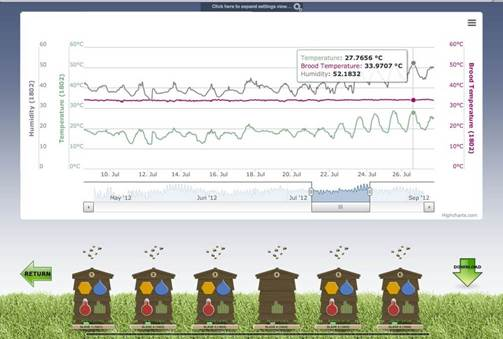
\includegraphics{arnia1.jpg}
\caption{\label{fig:arnia1} Interface du système d'arnia: comparaison des données d'une ruche}
\end{figure}

L'un des projets OpenSource est développé par Ken Meyer sur le site hackaday \cite{hackaday} et consiste à mesurer la température, l'humidité et le poids d'une ruche. Ce projet est encore en développement et plusieurs prototypes ont déjà été testés.

Il existe également un autre projet OpenSource sur le sujet. Il s'agit de Bzzz \cite{projetBzzz}, développé par le Fablab de Lannion. Ce système propose une supervision de la température intérieure, de la luminosité extérieure et la masse d'une seule ruche via un envoi de données périodique par SMS et par visualisation des données sur un portail en ligne. L'utilisateur pourra également configurer des alertes via le portail.

Enfin le dernier système existant que nous avons trouvé a été développé conjointement par le Fablab de Barcelone et Open Tech Collaborative, Denver, USA \cite{OpenBeehives}. Ce projet OpenSource, appelé Open Source BeeHive, ne s'adapte pas aux ruches classiques mais propose une architecture simple qui permet de construire sa propre ruche entièrement, comme on peut le voir sur les figures \ref{fig:OSBH2} et \ref{fig:OSBH}.

\begin{figure}[h]
\centering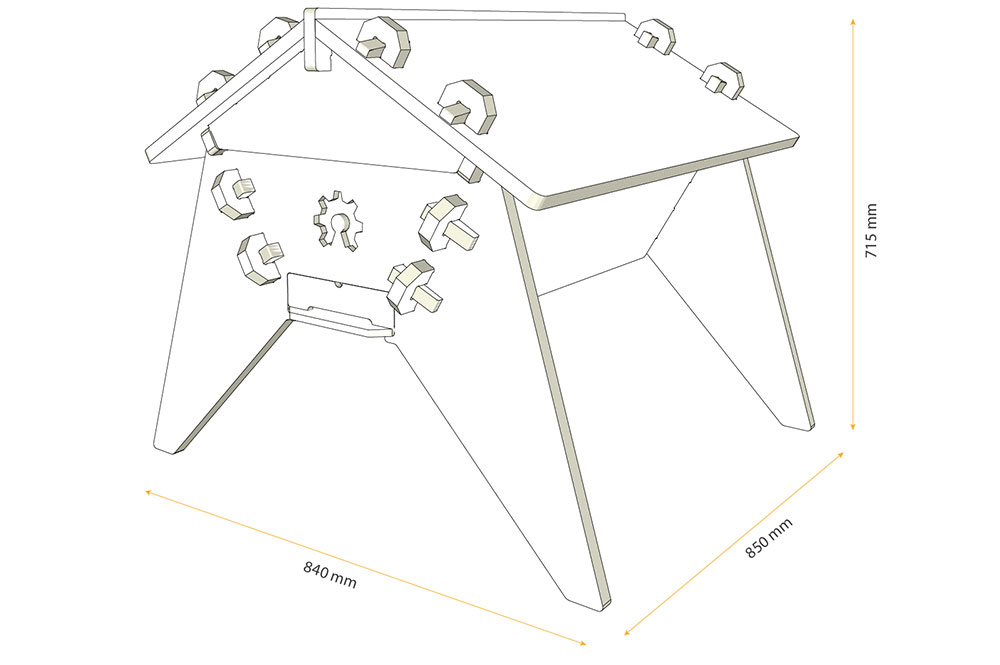
\includegraphics[scale=0.3]{OSBH.jpg}
\caption{\label{fig:OSBH} Modèle de ruche Open Source Beehive}
\end{figure}

\begin{figure}[h]
\centering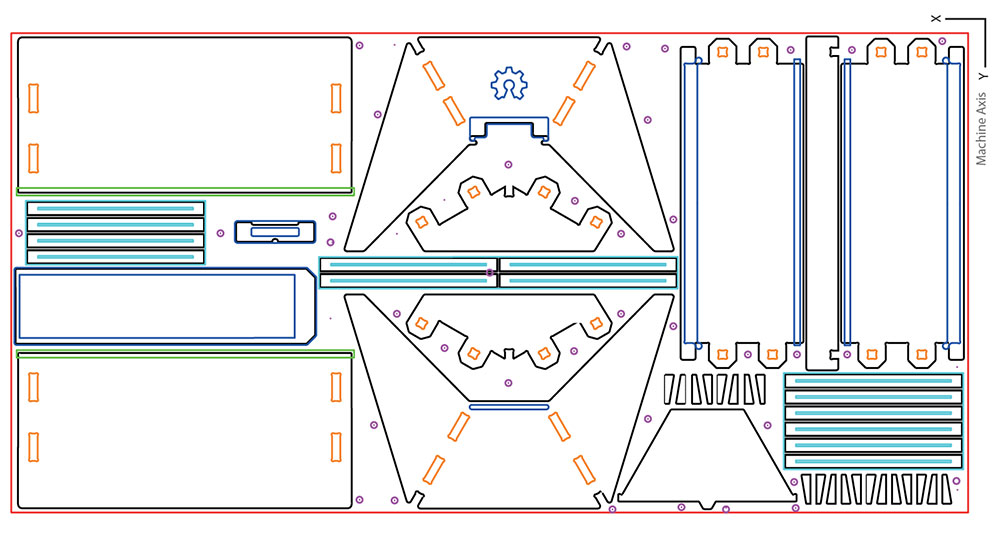
\includegraphics[scale=0.3]{OSBH2.jpg}
\caption{\label{fig:OSBH2} Plan de la ruche Open Source Beehive}
\end{figure}

Ensuite un kit de capteurs à installer permet de mesurer la température, l'humidité, l'intensité acoustique et le nombre d'abeilles via un capteur infrarouge. Les données seront ensuite visibles de tous sur la plateforme Smart Citizen.

Nous n'avons pas détaillé ici tous les projets que nous avons trouvés du fait de leur grand nombre. Cependant nous nous sommes intéressés à ceux qui présentaient un intérêt pour le système que nous voulons développer. 

Concernant le traitement sonore, le site internet Beesource comporte une description complète du système Apidictor \cite{apidictor}. Ce système permet de filtrer le son émit par une ruche pour prévoir un essaimage. Un schéma du montage électrique ainsi qu'un texte expliquant quelles fréquences sont surveillées et quelles méthodes ont été utilisées pour vérifier le bon fonctionnement de ce système sont également présents. Nous ne réutiliserons pas le montage proposé, car le traitement du signal sonore se fera de manière informatisée, en revanche le travail effectué pour savoir quelles fréquences sont à surveiller nous sera utile. \\

A propos de la transmission de l'information à l'apiculteur, deux moyens sont très souvent utilisés: un site internet sécurisé et une application pour smart-phone. Concernant le site internet, celui de la société Arnia nous a semblé complet et clair. Pour l'application smart-phone, l'entreprise américaine B-Ware en a mis une au point mettant bien en avant le tableau de bord, l'affichage de l'historique des paramètres de la ruche et la personnalisation des alertes en laissant même l'apiculteur définir lui même les seuils de déclenchement des avertissements comme nous pouvons le voir sur la figure \ref{fig:application}.   

\begin{figure}[h]
\centering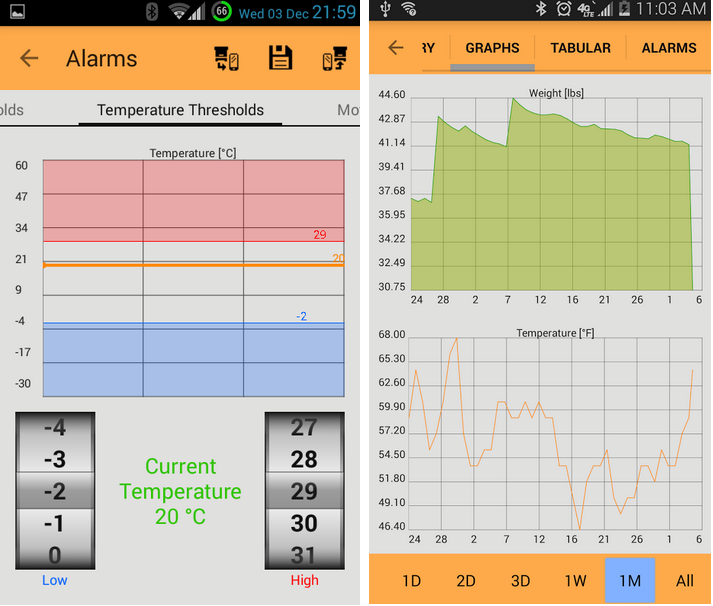
\includegraphics[scale=0.5]{Bee_app.png}
\caption{\label{fig:application} Capture d'écran de l'application B-Ware}
\end{figure} 

La société BeeWise d'origine française a développé un système d'alimentation écologique à l'aide de panneaux solaires connectés au  boitier regroupant les cartes électroniques pour le traitement des données et de transmission \cite{BeeWise}. Il suffirai juste de la fixer sur le couvercle de la ruche en prenant soin d'étudier l'orientation adéquate au préalable comme sur la figure \ref{fig:solar}. Cette solution semble être la plus répandue car elle est également utilisée par les développeurs de l'ApiScan, un système de comptage de d'abeilles installé sur la planche d'envol pour minimiser la gène occasionnée.    

\begin{figure}[h]
\centering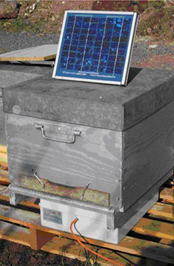
\includegraphics[scale=0.9]{solar.png}
\caption{\label{fig:solar} Système de panneau solaire installé sur une ruche}
\end{figure} 

Les recherches sur l'exploitation des ruchers nous a mené à comprendre que l'un des principaux risques pour les apiculteurs est le vol de ruche. Cette pratique s'est très largement répandue ces dernières années. C'est pour cela que la société Apimiel met à disposition un système GPS pour permettre à l'apiculteur de connaitre en temps réel la position de ses ruches \cite{Apimiel}. Au moindre déplacement, l'apiculteur recevra une alerte SMS. Compte tenu de sa taille, le traceur GPS devra se trouver à l'extérieur de la ruche mais il existe aussi des versions plus petites que l'on peut directement placer dans la ruche comme sur la figure \ref{fig:gps}. C'est ce que Michel BOCQUET, ingénieur agronome, propose sur son blog. Néanmoins, son objectif final est d'étudier le comportement des abeilles pour mieux comprendre celui de notre environnement et non commercialiser son projet aux apiculteurs. Le coût du matériel n'est donc pas pris en compte. 

\begin{figure}[h]
\centering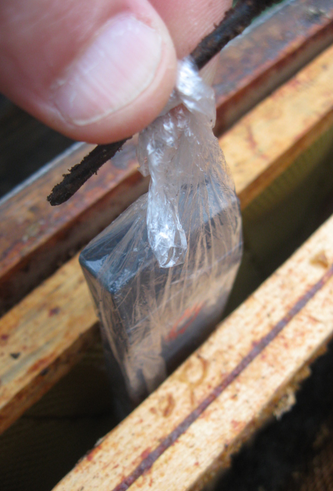
\includegraphics[scale=0.5]{gps.png}
\caption{\label{fig:gps} Système GPS placé dans la ruche}
\end{figure} 
     

   



%----------------------------------------------------------------------------------------
%	PART II 
%----------------------------------------------------------------------------------------
\part{Cahier des charges fonctionnel}
\chapter{Ingénierie des exigences}
\section{Approche Top-Down}
\vspace{1.5cm}
Dans cette partie nous allons analyser notre système avec une approche Top-Down. Cela signifie que nous adopterons une démarche de conception descendante. Pour cela nous avons tracé le diagramme "bête à cornes", que l'on peut voir sur la figure \ref{fig:beteacorne}. Il permet de représenter graphiquement l'expression du besoin. Comme on peut le voir sur le diagramme, le système BMONS rend service aux apiculteurs en agissant sur une ou plusieurs ruches. Il a pour but d'aider la surveillance d'un rucher et d'avertir l'apiculteur en cas de problème.


\begin{figure}[h!]
\centering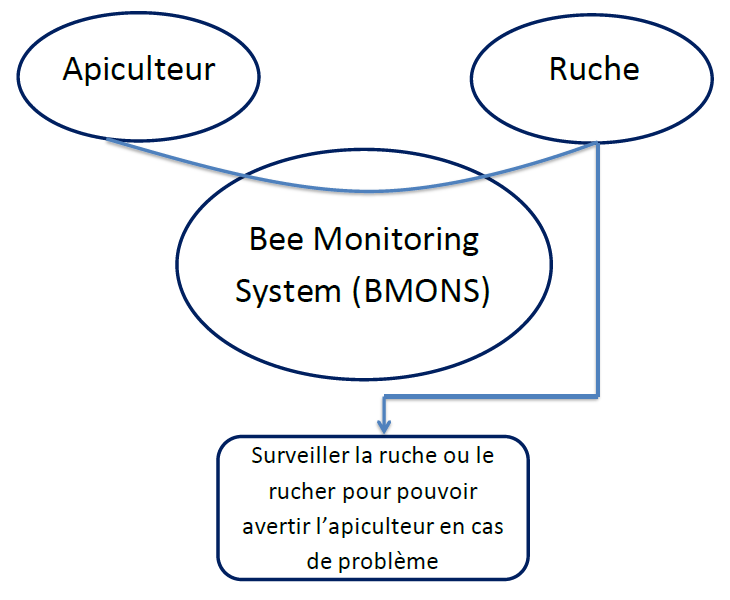
\includegraphics[scale=0.5]{BeteACornesBMONS.png}
\caption{\label{fig:beteacorne} Diagramme "bête à cornes" du système BMONS}
\end{figure}

Le diagramme pieuvre, \ref{fig:diagpieuvre1} et \ref{fig:diagpieuvre2}, nous permet ensuite de faire apparaître les fonctions principales du système. On peut aussi y retrouver les fonctions de services et de contraintes.

 
\begin{figure}[h!]
\centering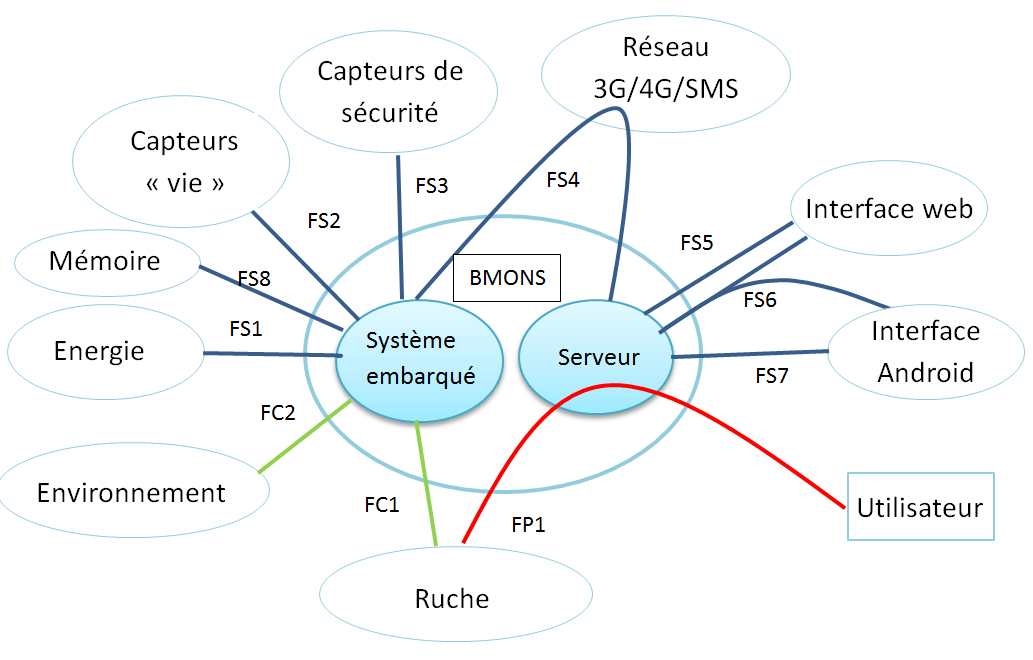
\includegraphics[scale=0.6]{pieuvre1.png}
\caption{\label{fig:diagpieuvre1} Diagramme pieuvre du système BMONS}
\end{figure}

\begin{figure}[h!]
\centering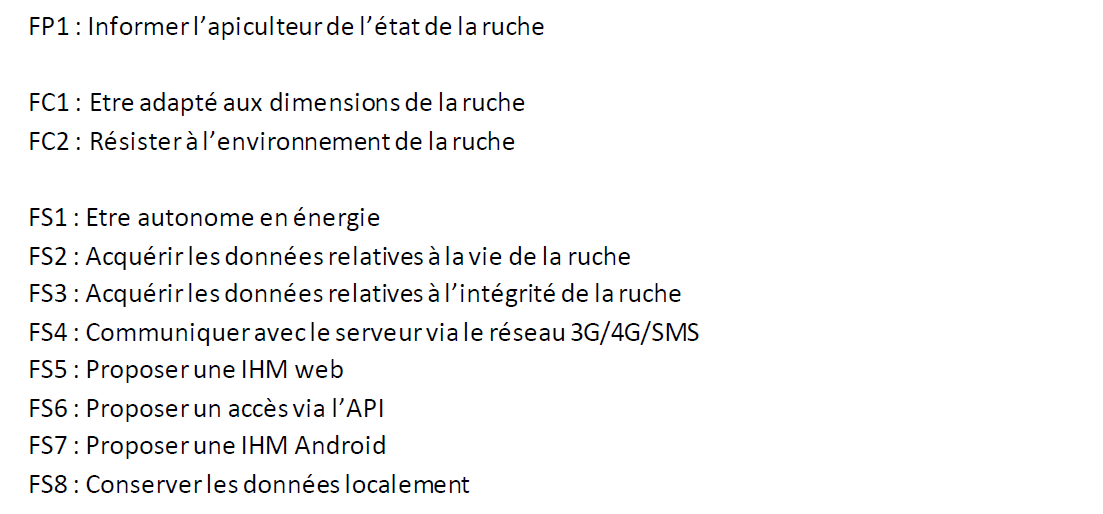
\includegraphics[trim = 1cm 0.5cm 13cm 1cm,scale=0.6]{pieuvre2.png}
\caption{\label{fig:diagpieuvre2} Légende diagramme pieuvre du système BMONS}
\end{figure}

\clearpage

\section{Approche Bottom-Up}

\vspace{1.5cm}
Nous allons maintenant adopter la démarche inverse, mais néanmoins complémentaire, de l'approche Top-Down. Il s'agit de l'approche Bottom-Up. C'est une démarche de conception ascendante qui va nous permettre d'avoir une vision plus globale du système. On peut voir sur \ref{fig:exi1} et \ref{fig:exi2} les exigences issues de cette analyse.

 
\begin{figure}[h!]
\centering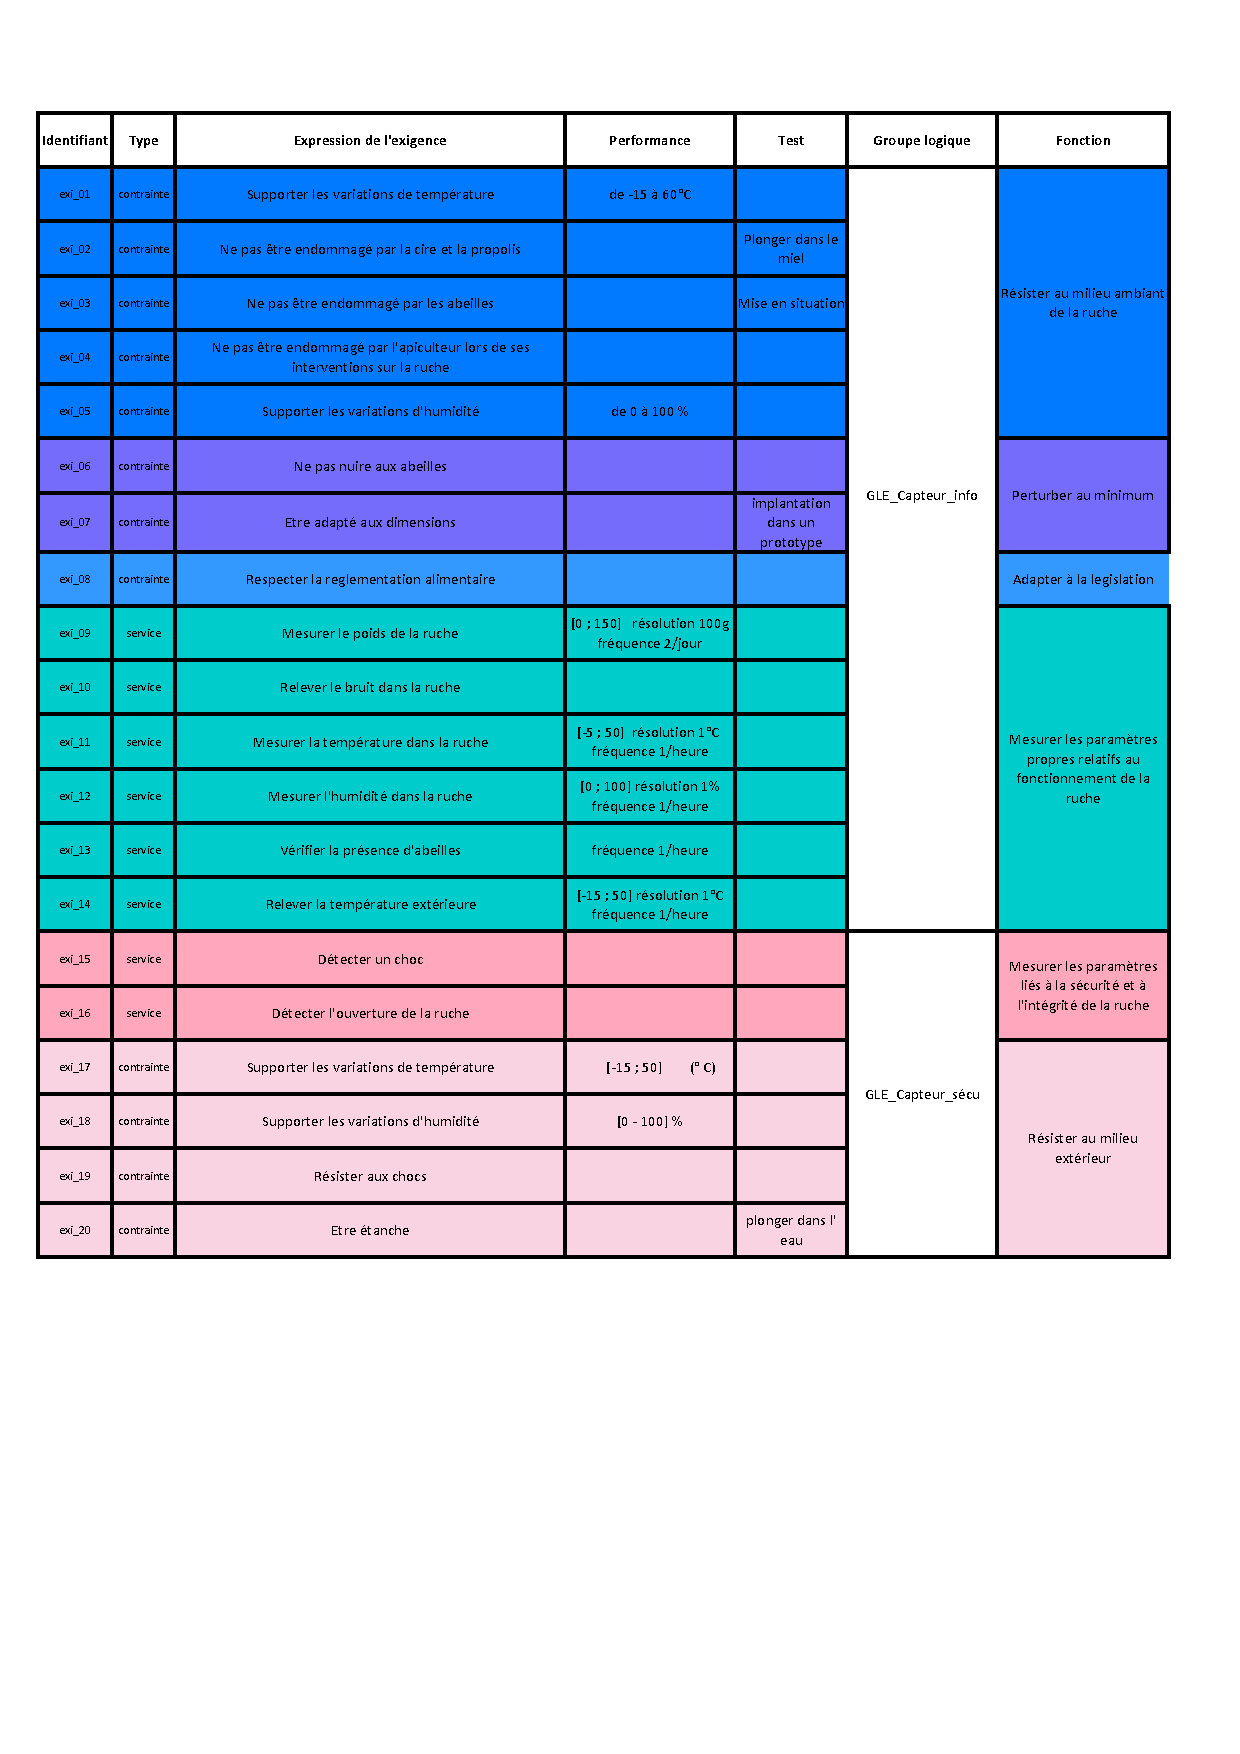
\includegraphics[trim = 1cm 8.7cm 1cm 1cm,scale=0.8]{Exigences_du_Projet_1.pdf}
\caption{\label{fig:exi1} Exigences issues de l'approche Bottom-Up (1/2)}
\end{figure}

 
\begin{figure}[h!]
\centering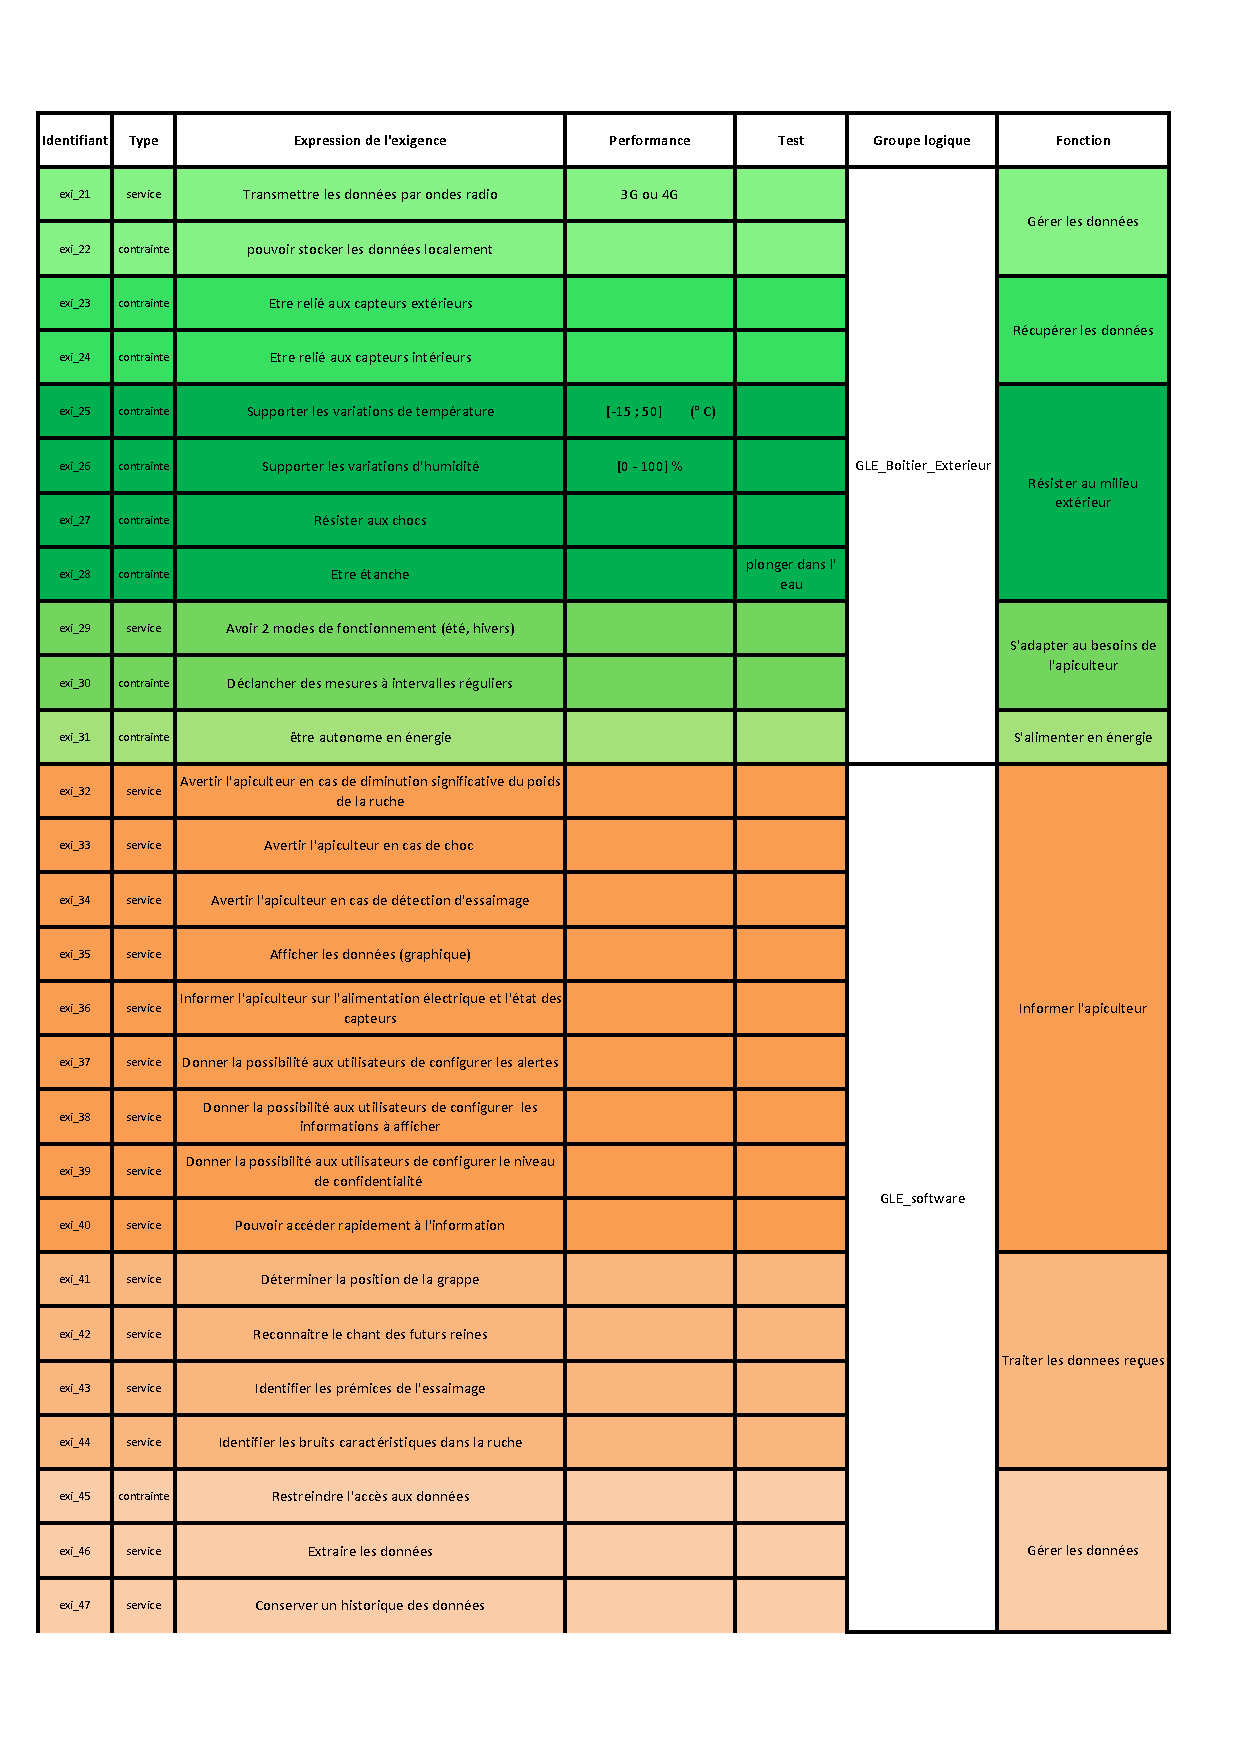
\includegraphics[trim = 1cm 2cm 1cm 1cm,scale=0.8]{Exigences_du_Projet_2.pdf}
\caption{\label{fig:exi2} Exigences issues de l'approche Bottom-Up (2/2)}
\end{figure}

\clearpage

\section{Fonctions métiers du système}
\vspace{1.5cm}

Après avoir réalisé une approche du point de vue "concepteur" du système, nous allons maintenant nous intéresser à la formulation des fonctions qu'un apiculteur souhaiterai avoir pour pouvoir suivre l'évolution de son rucher. Ces fonctions métiers ont été discutées avec notre client, monsieur Singhoff. Elles sont représentées sur les figures \ref{fig:exi1,exi2,exi3,exi4} en annexe dont la figure \ref{fig:exi1text} est un extrait.


\begin{figure}[h!]
\centering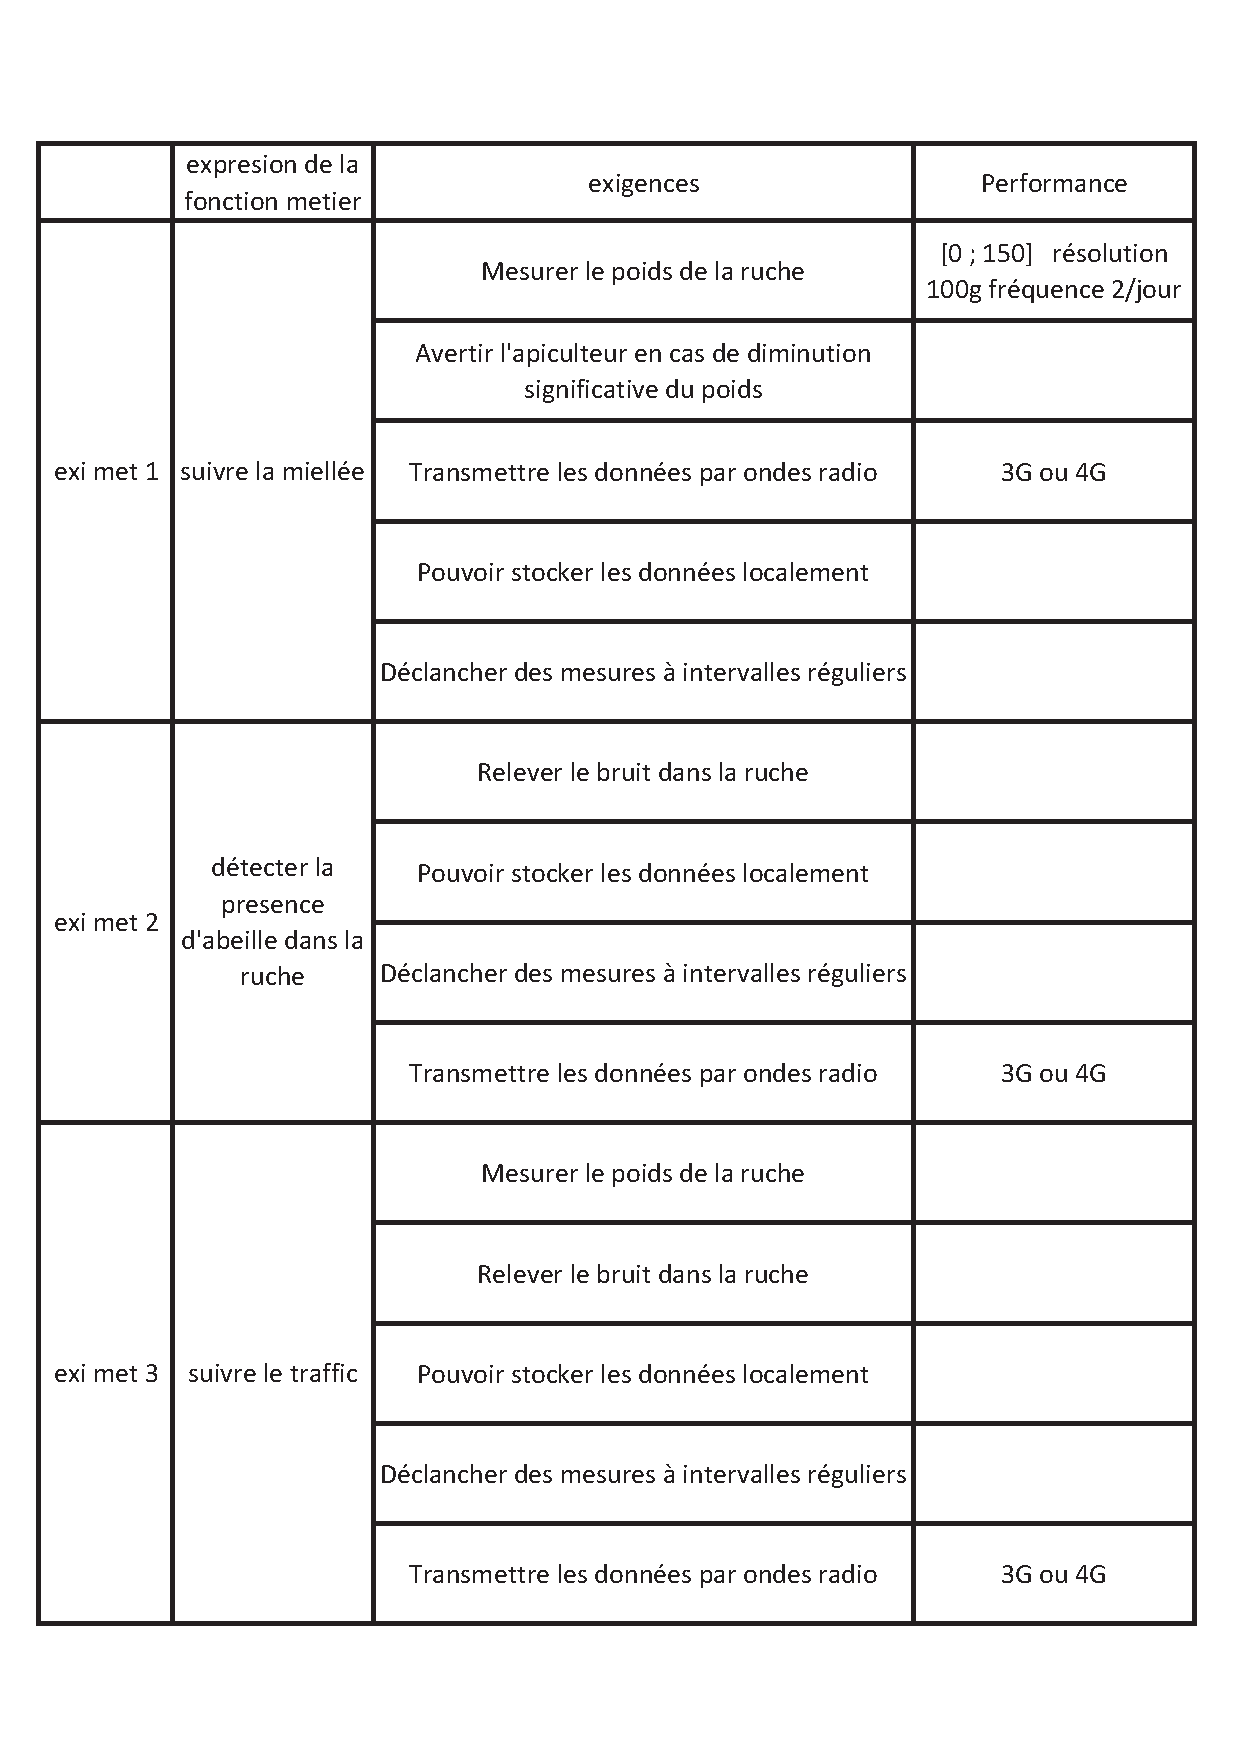
\includegraphics[trim = 1cm 2cm 1cm 1cm,scale=0.65]{Exigences1.pdf}
\caption{\label{fig:exi1text} Fonctions métiers du système (1/4)}
\end{figure}



\clearpage


\chapter{Architecture fonctionnelle}

L'étude de la spécification fonctionnelle trois axes a permis d'établir l'architecture fonctionnelle du système qui est représentée sur la figure \ref{fig:anaFonc}.
Ce schéma résume les interactions entre chaque partie: Bee Monitor qui regroupe l'ensemble des capteurs, la carte Arduino ainsi que la carte SSD pour l'enregistrement local des données, le module de transmission et le système d'alimentation rendant notre projet autonome en énergie et le serveur. Chaque acteur interagissant avec le système est également représenté: Les abeilles/ruche, l'apiculteur et l'environnement.   
  

\begin{figure}[h]
\centering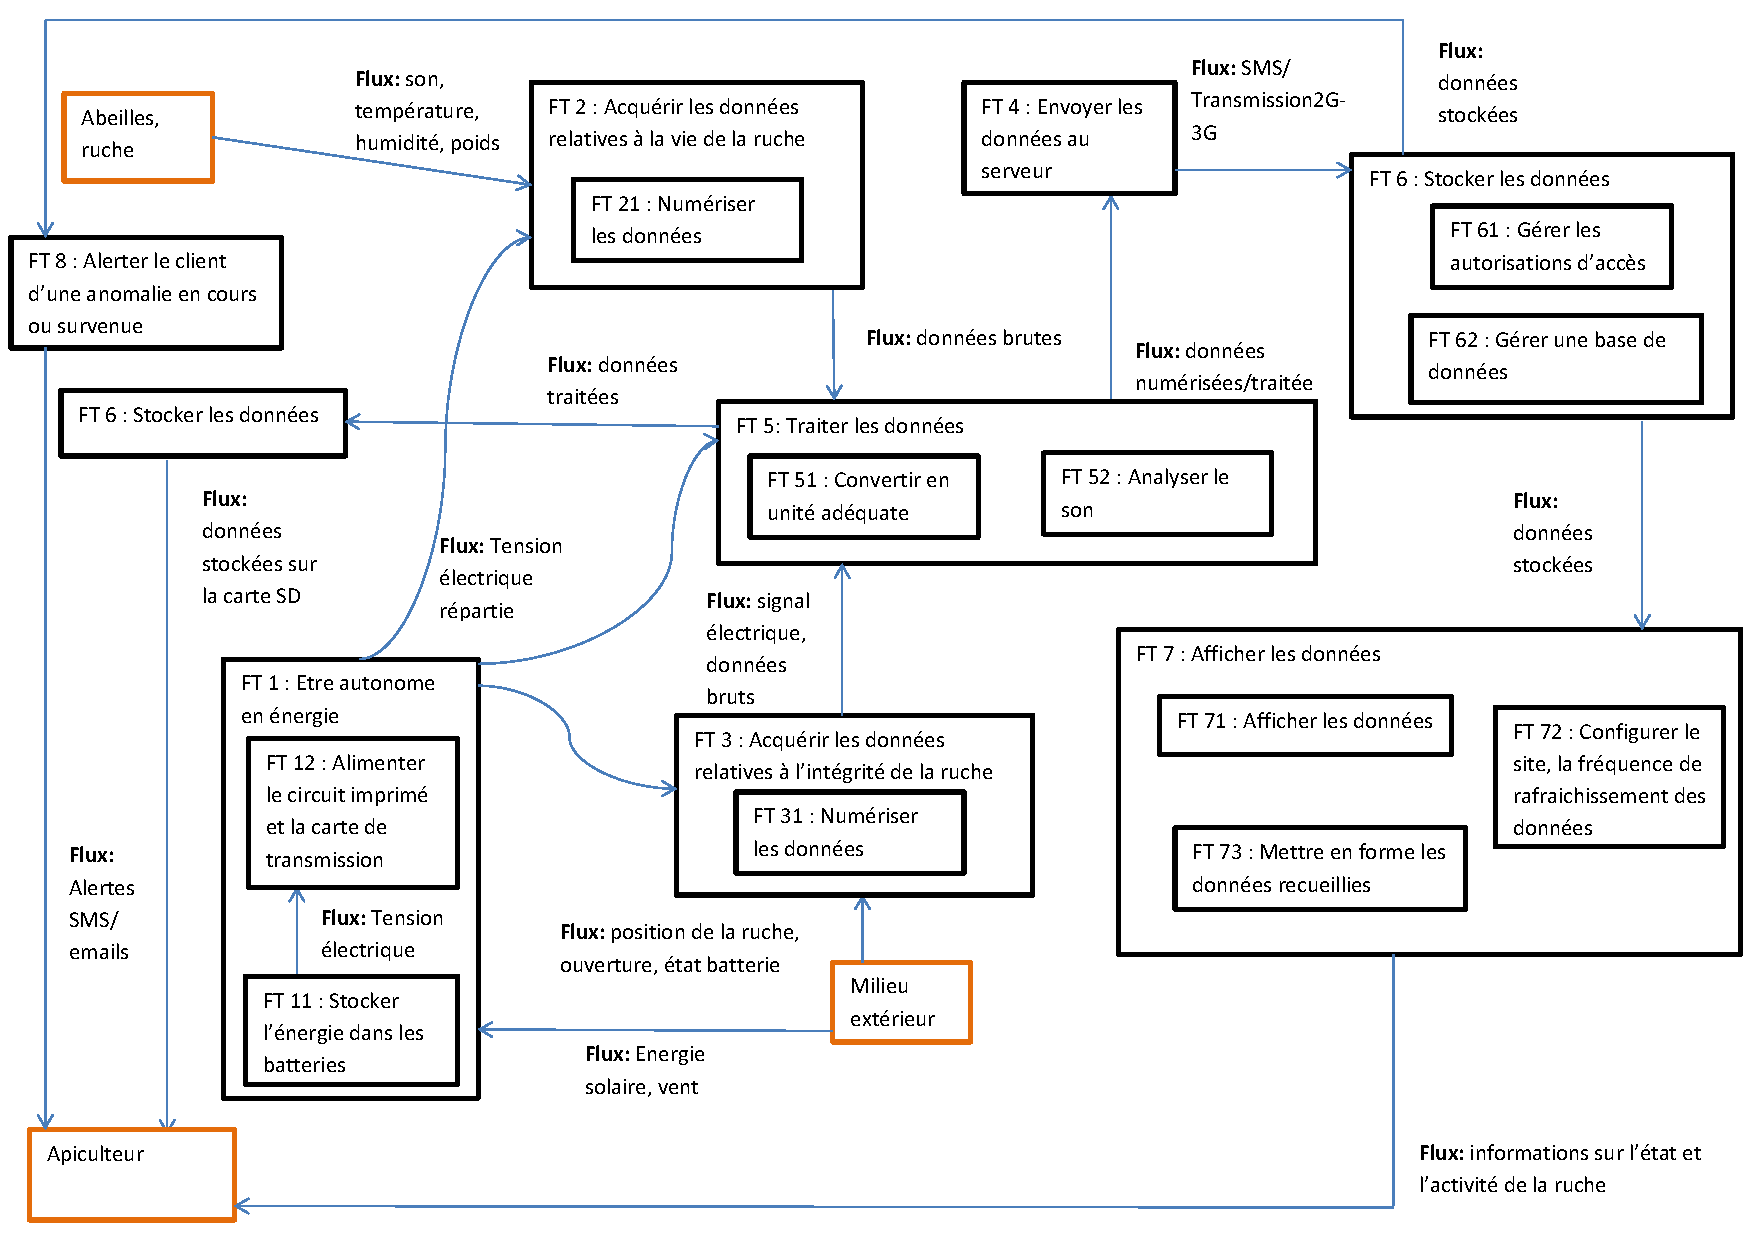
\includegraphics[scale=0.5]{analyseFonctionelle1.pdf}
\caption{\label{fig:anaFonc} Architecture fonctionnelle}
\end{figure}    



\chapter{Architecture physique}

\section{Architecture physique}


%----------------------------------------------------------------------------------------
%	PART III 
%----------------------------------------------------------------------------------------
\part{Organisation}
\chapter{Méthodes de travail}

% Méthodes de travail
% Organisation temporelle, spatiale, humaine 
% interactions des membres de l’équipe projet
% interactions avec les encadrants
% interactions avec les tiers

Tout au long du projet notre méthode de travail a changée. Au fur et à mesure que les séances s'enchainaient, et en prenant en compte les conseils qui nous ont été donnés (notamment à propos du carnet de bord et des objectifs à court terme) notre méthode de travail a tendu vers la suivante : \\ \\
De manière générale, toute l'équipe du projet BMONS travaille dans la même salle pour faciliter la communication entre les membres du groupe. Une séance de travail commence par l'ouverture personnelle des mails de chacun, puis le groupe se réunit pour définir les objectifs de la matinée, ensuite chacun choisit la partie il va avancer. Le travail se fait en général seul ou en binôme et des points d'avancement sont faits à l'oral tout au long de la séance. Parfois des tâches comme la prise en main d'un logiciel ou la compréhension d'un diagramme sont faites en dehors des séances, mais la majeure partie du travail s'effectue lors du temps alloué au projet. \\ \\
Les réunions avec les encadrants et les intervenants extérieurs se déroulent dans des salles de l'ENSTA Bretagne équipées d'un vidéo projecteur et en présence de la totalité de l'équipe BMONS. Ces séances sont organisées à l'avance, les points sur lesquels des précisions sont nécessaires sont mis en avant avant la séance et des questions précises sont préparées. Cela permet de guider la réunion et de ne pas perdre de temps sur des points déjà vus. Chacun a son rôle lors de ces réunions, la prise de notes, le dialogue avec l'intervenant et la rédaction du compte rendu sont ainsi facilités.


 

\chapter{Outils pour les échanges}

% Quels sont les outils qui nous permettent de travailler ensemble ?

Les outils qui nous ont permis de travailler ensemble et de partager nos fichiers ont également changés au cours du temps. 
Avant les premiers ateliers techniques, particulièrement celui sur github, nous partagions nos résultats sur le oneDrive d'office 365. \\

\chapter{Répartition des tâches dans le temps}


% WBS et diagramme de Gantt




%----------------------------------------------------------------------------------------
%	PART IV 
%----------------------------------------------------------------------------------------
\part{Présentation des réalisations}
\chapter{Le cadre de mesure}

Le cadre de mesure a été réalisé en bois. Les dimensions ont été choisi afin de limiter au maximum l'encombrement et en concertation avec notre client, M. Singhoff, afin que l'environnement des abeilles ne soit pas perturbé. Sa hauteur maximale a été fixé à 1 cm. Cette taille lui permet de rester à la fois discret une fois monté sur la ruche et de faciliter les actions de l'apiculteur car il aura juste à retirer un seul élément.\\
Cette contrainte nous a conduit à réétudier la conception du cadre pour finalement placer les capteurs entre une couche de bois et une couche de métal ce qui le rendra plus rigide et moins épais qu'entre deux couches de bois.\\
Le cadre a été dessiné sur Catia puis fabriqué grâce à la fraiseuse de l'ENSTA Bretagne en deux parties qui viendront s'emboiter lors du montage.\\

\begin{figure}[h!]
\centering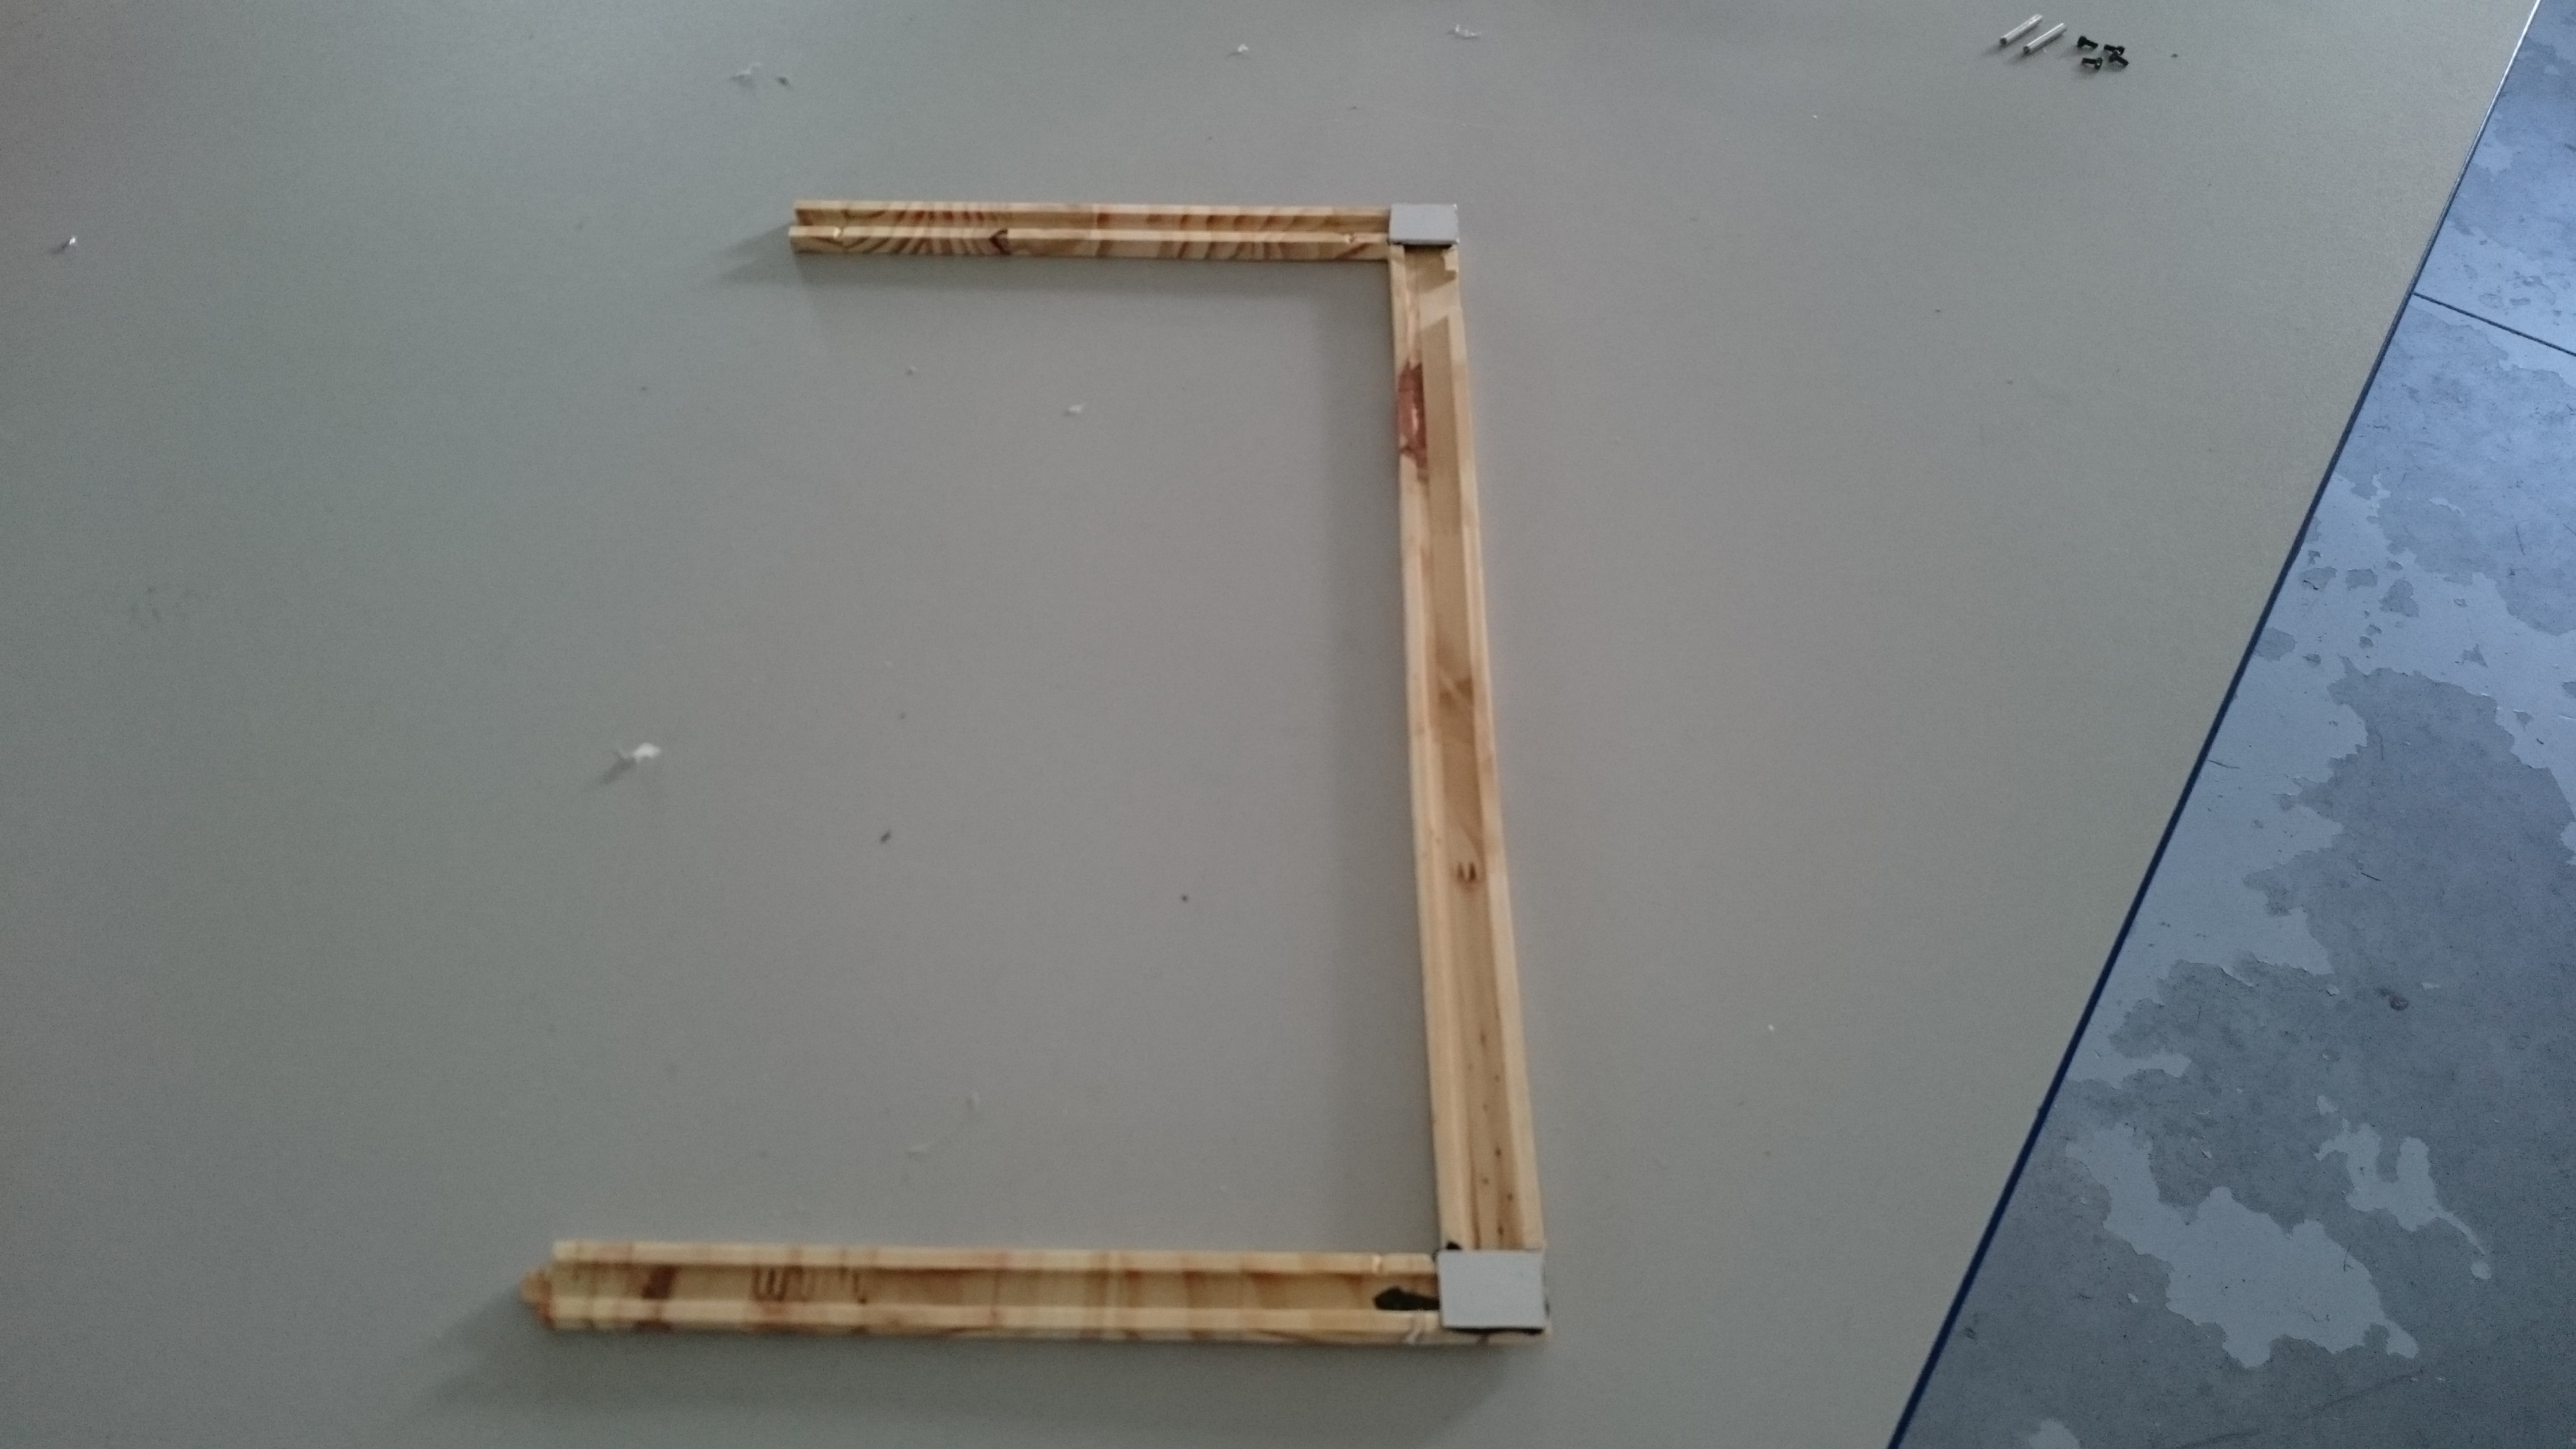
\includegraphics[trim= 0cm 0cm 0cm 0cm,scale=0.08]{cadre.jpg}
\caption{\label{fig:cote1} Schéma d'une des deux parties du cadre de mesure}
\end{figure}

\clearpage

\section{Intégration des capteurs}

Nous avons décidé de positionner 14 capteurs sur notre cadre afin de recueillir 5 paramètres:\\

\indent - 6 thermistances \\
\indent - 4 capteurs de pression \\ 
\indent - 2 tilt \\ 
\indent - 1 capteur de son \\
\indent - 1 capteur d'humidité \\

Ces capteurs ont été disposé comme sur la figure \ref{fig:face} présenté dans le chapitre 5: Architecture physique. Chaque capteur est relié à 2 ou 3 fils pour ceux qui sont déjà installé sur une carte. C'est le cas pour les trois derniers capteurs ci-dessus. Pour les thermistances et les capteurs de pressions, nous les avons monté sur une carte en série avec des résistances de 10 kOhm pour les premiers et 1.8 kOhm pour les second. Le choix d'une résistance faible pour les capteurs de pression nous permet d'avoir une meilleur précision au niveau de la plage de masse qui nous intéresse. Ces capteurs de poids permettrons soit de récupérer le poids de la ruche et ainsi suivre l'évolution de la colonie, soit celle des hausse et donc suivre la miellée.\\

Avant d'être intégrés au cadre, les capteurs ont été testé individuellement. Les capteurs de pression qui permettront de déterminer le poids de la ruche ont notamment dû être étalonnés. Nous avons réalisé cette manipulation dans un des laboratoires de mécanique de l'école. Comme nous pouvons le voir sur la figure \ref{fig:pression}, nous avons placé chaque capteur de pression sur une machine capable d'exercer une gamme prédéfinie de pressions sur la zone de test. Nous avons relevé la réponse du capteur, une tension entre 0 et 5 volts, pour chaque échantillon lors de trois séries de mesures. Ces séries étaient composées d'un ensemble d'échantillons répartis comme suit: 20 valeurs croissantes de force de 0 à 100 Newtons puis 20 valeurs décroissantes de 100 à 0 Newton.

\begin{figure}[h]
\centering
	\subfigure{
		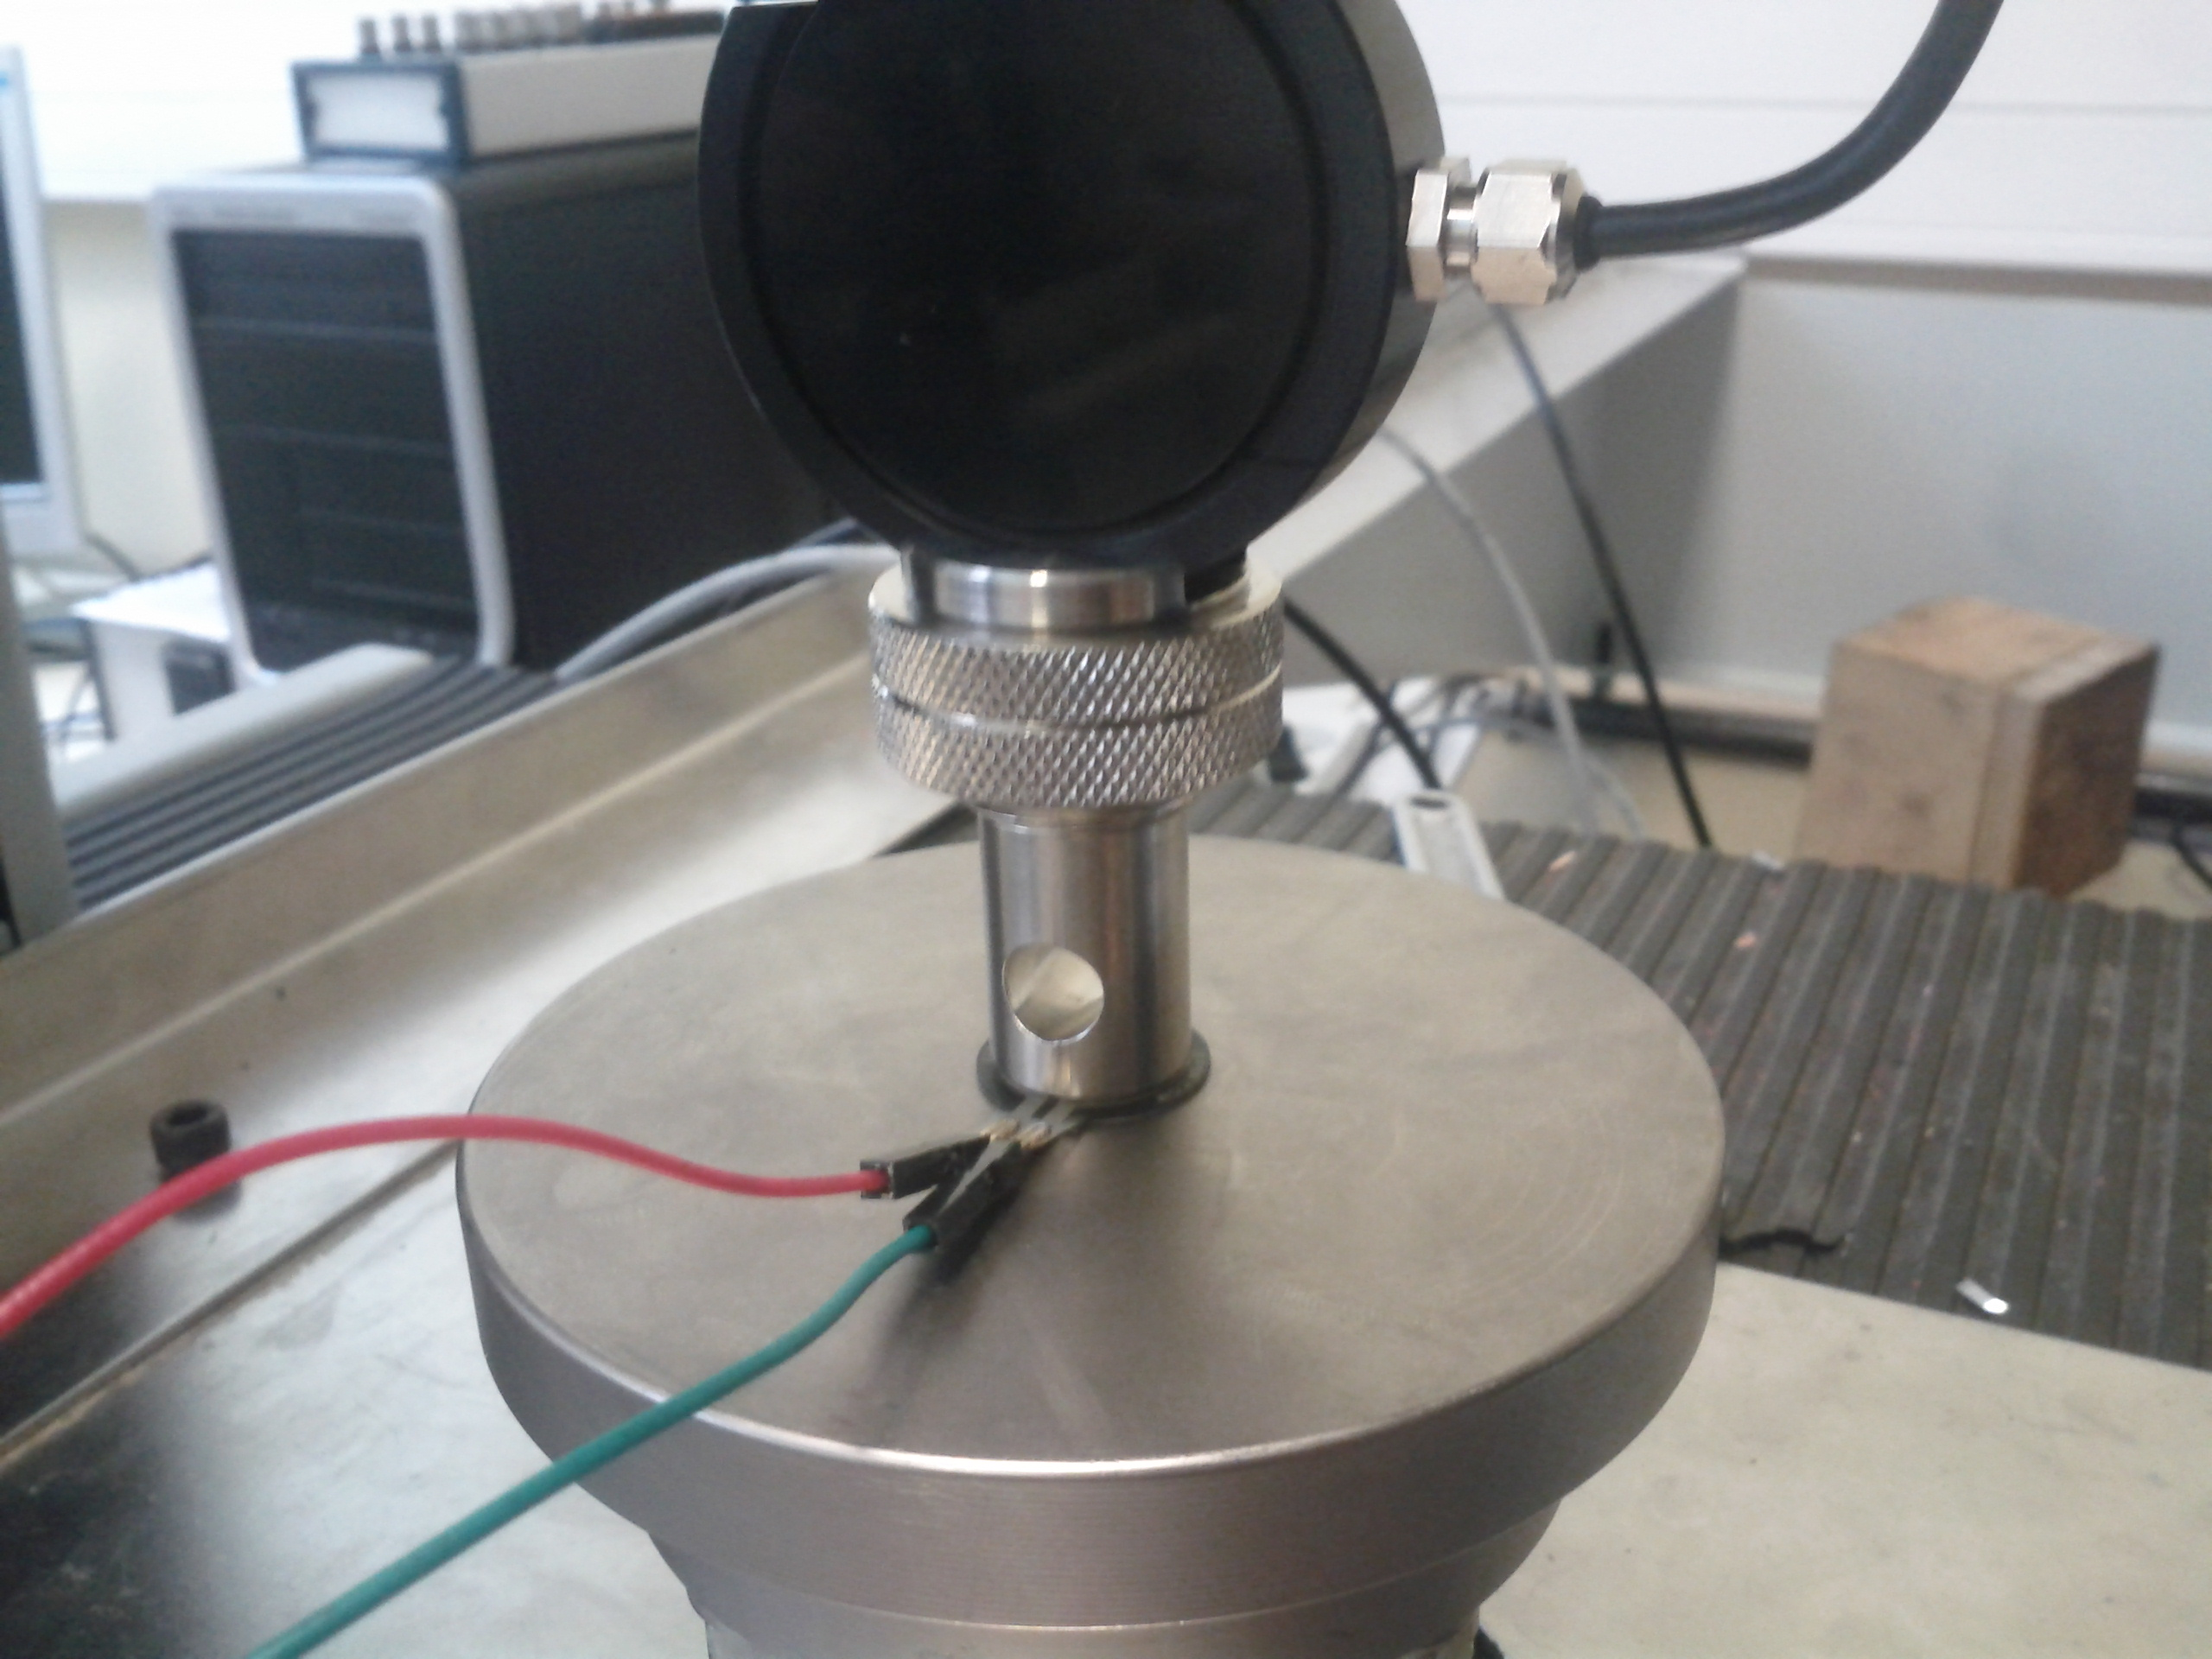
\includegraphics[scale=0.08]{testPression1.jpg}
		}
	\quad
	\subfigure{
		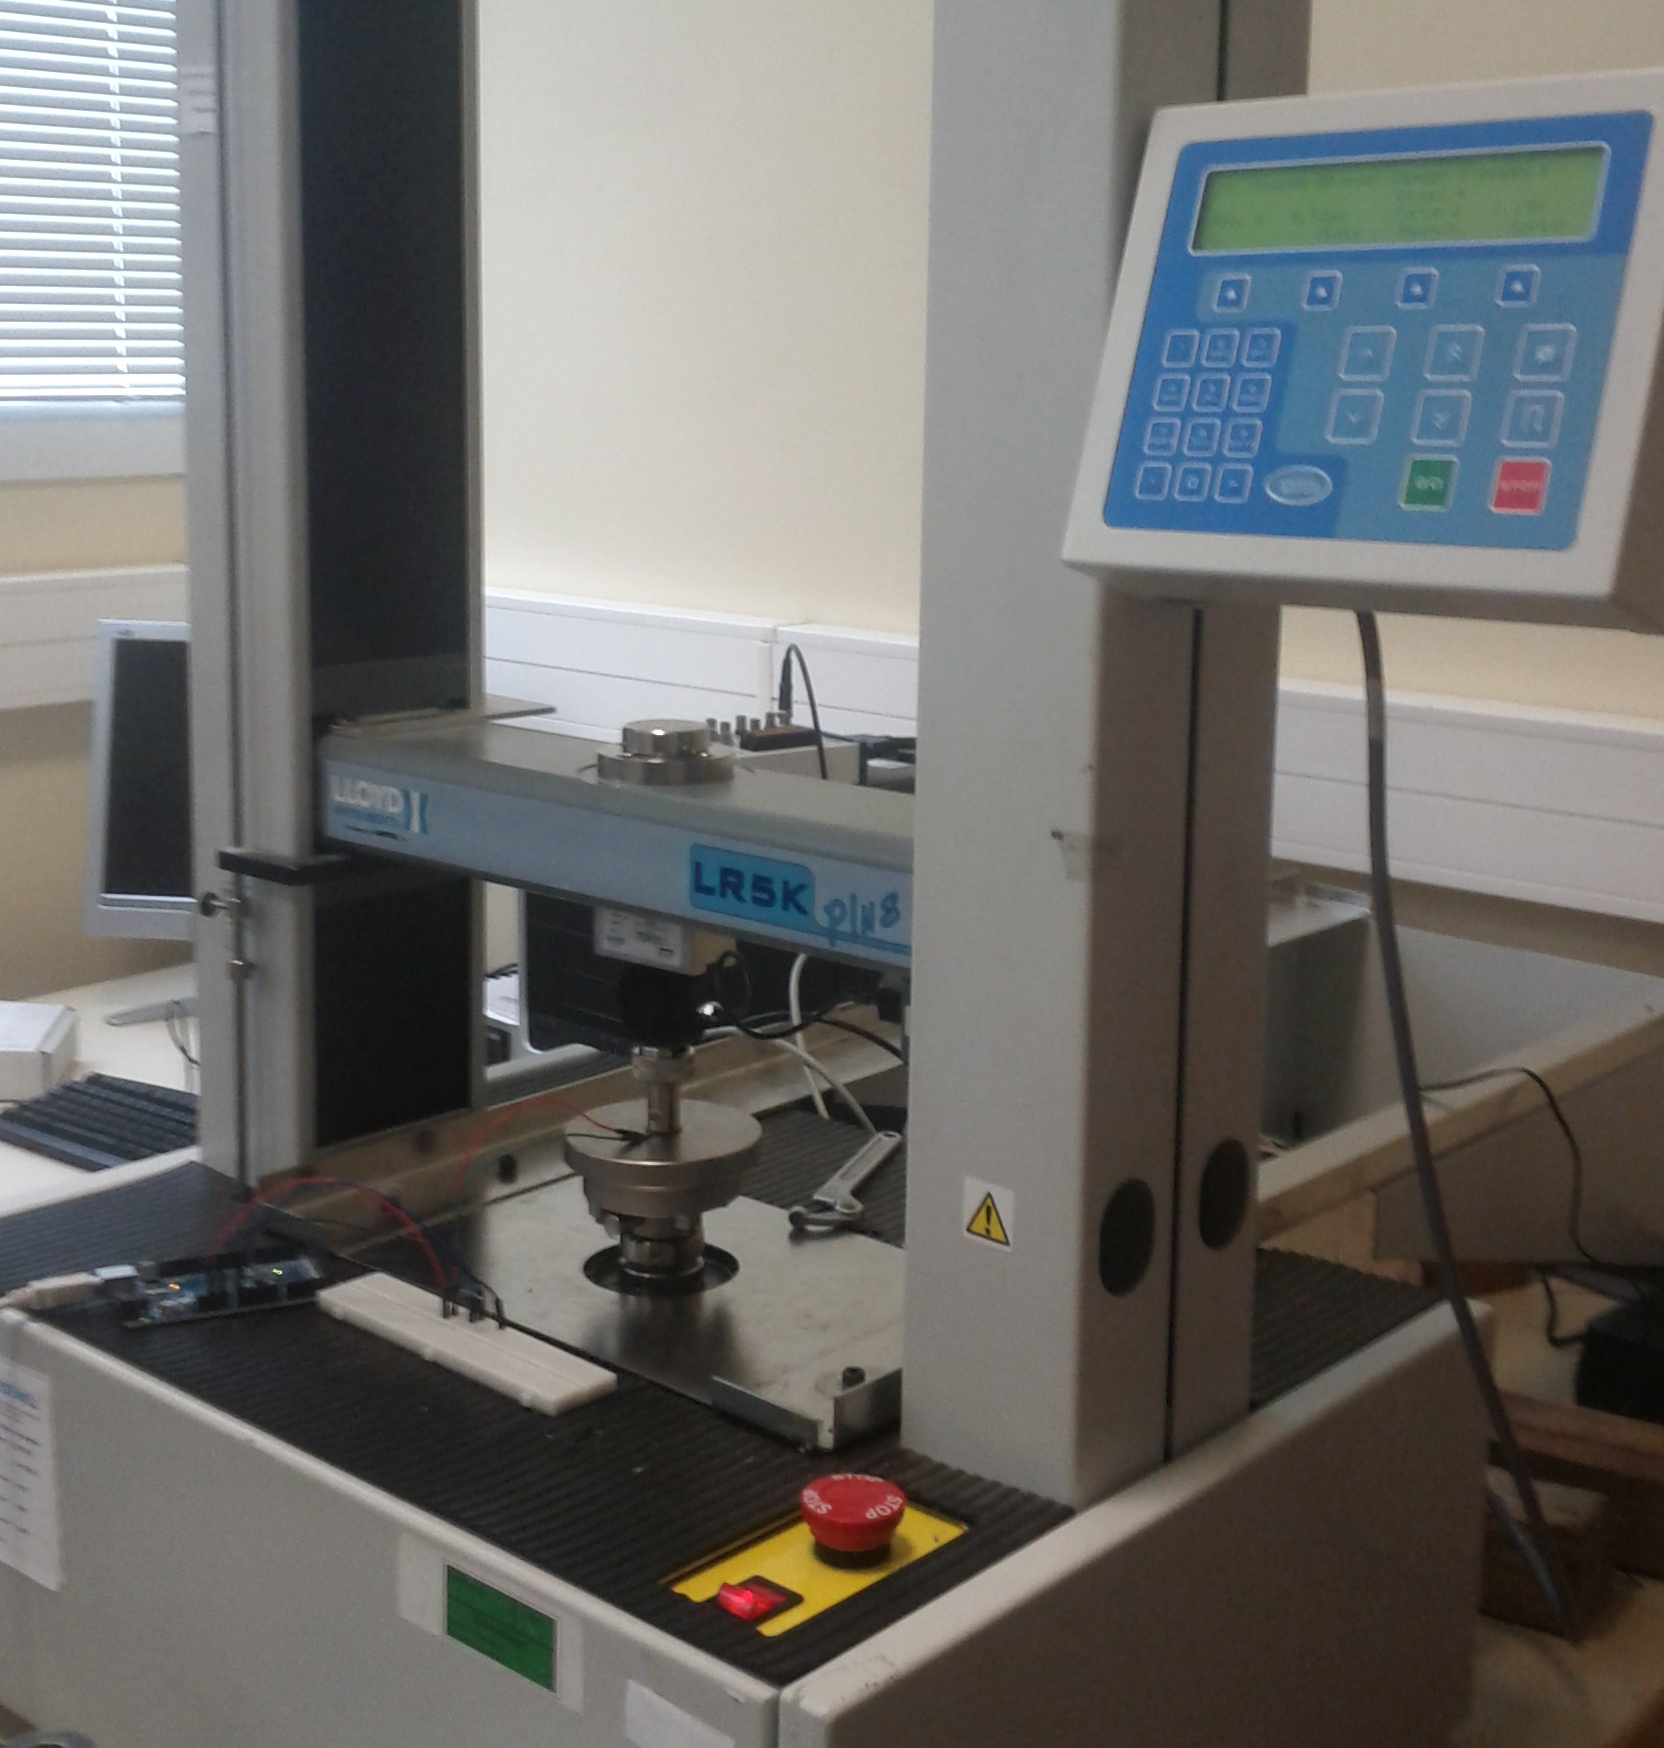
\includegraphics[scale=0.1]{testPression2.jpg}
		}
	\caption{\label{fig:pression} \'Etalonnage des capteurs de pression dans un laboratoire de mécanique de l'ENSTA Bretagne }
\end{figure}


L'ensemble des valeurs obtenues nous a permis de tracer la courbe qui nous donne une mesure de masse en fonction de la tension en sortie du capteur, voir figure \ref{fig:courbe}. Nous avons ensuite obtenu une équation de cette courbe de tendance. L'équation de cette courbe est de type polynomiale de degré 6 et $R²=0.96$. Comme les calculs de conversion ne seront pas effectués par l'Arduino mais par le serveur, la forme de cette équations n'est pas problématique. Nous avons également vérifié que tous les capteurs de pression suivent bien la même loi. Nous avons donc une formule unique de conversion de la tension de sortie en masse appliquée.

\begin{figure}[!h]
\centering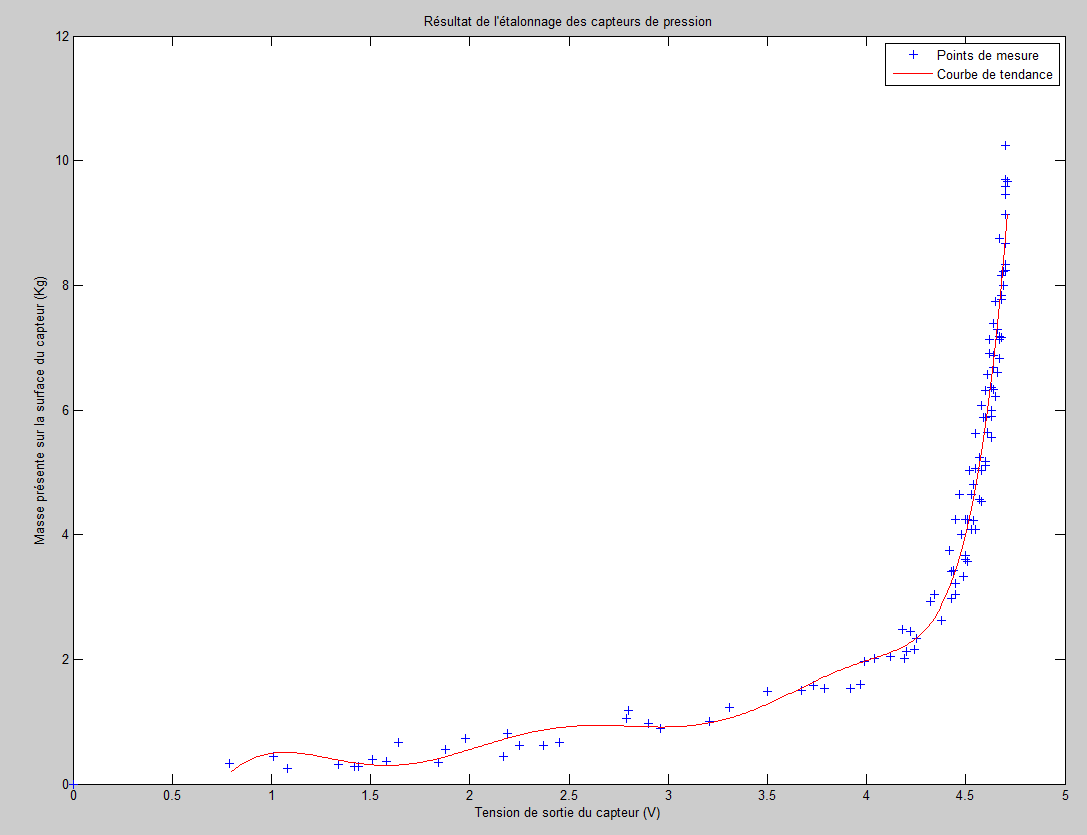
\includegraphics[scale=0.3]{courbe.png}
\caption{\label{fig:courbe} Courbe de tendance obtenue par l"étalonnage des capteurs de pression}
\end{figure} 

Les capteurs de pression se situent au niveau des 4 coins du cadre avec une position très légèrement sur-élevée afin que le matériel reposent uniquement sur ces derniers comme nous pouvons le voir sur la figure \ref{fig:pression2}. Ces capteurs sont positionnés entre 2 plaques rigides en métal afin de limiter les erreurs de mesures. 

\clearpage

\begin{figure}[h!]
\centering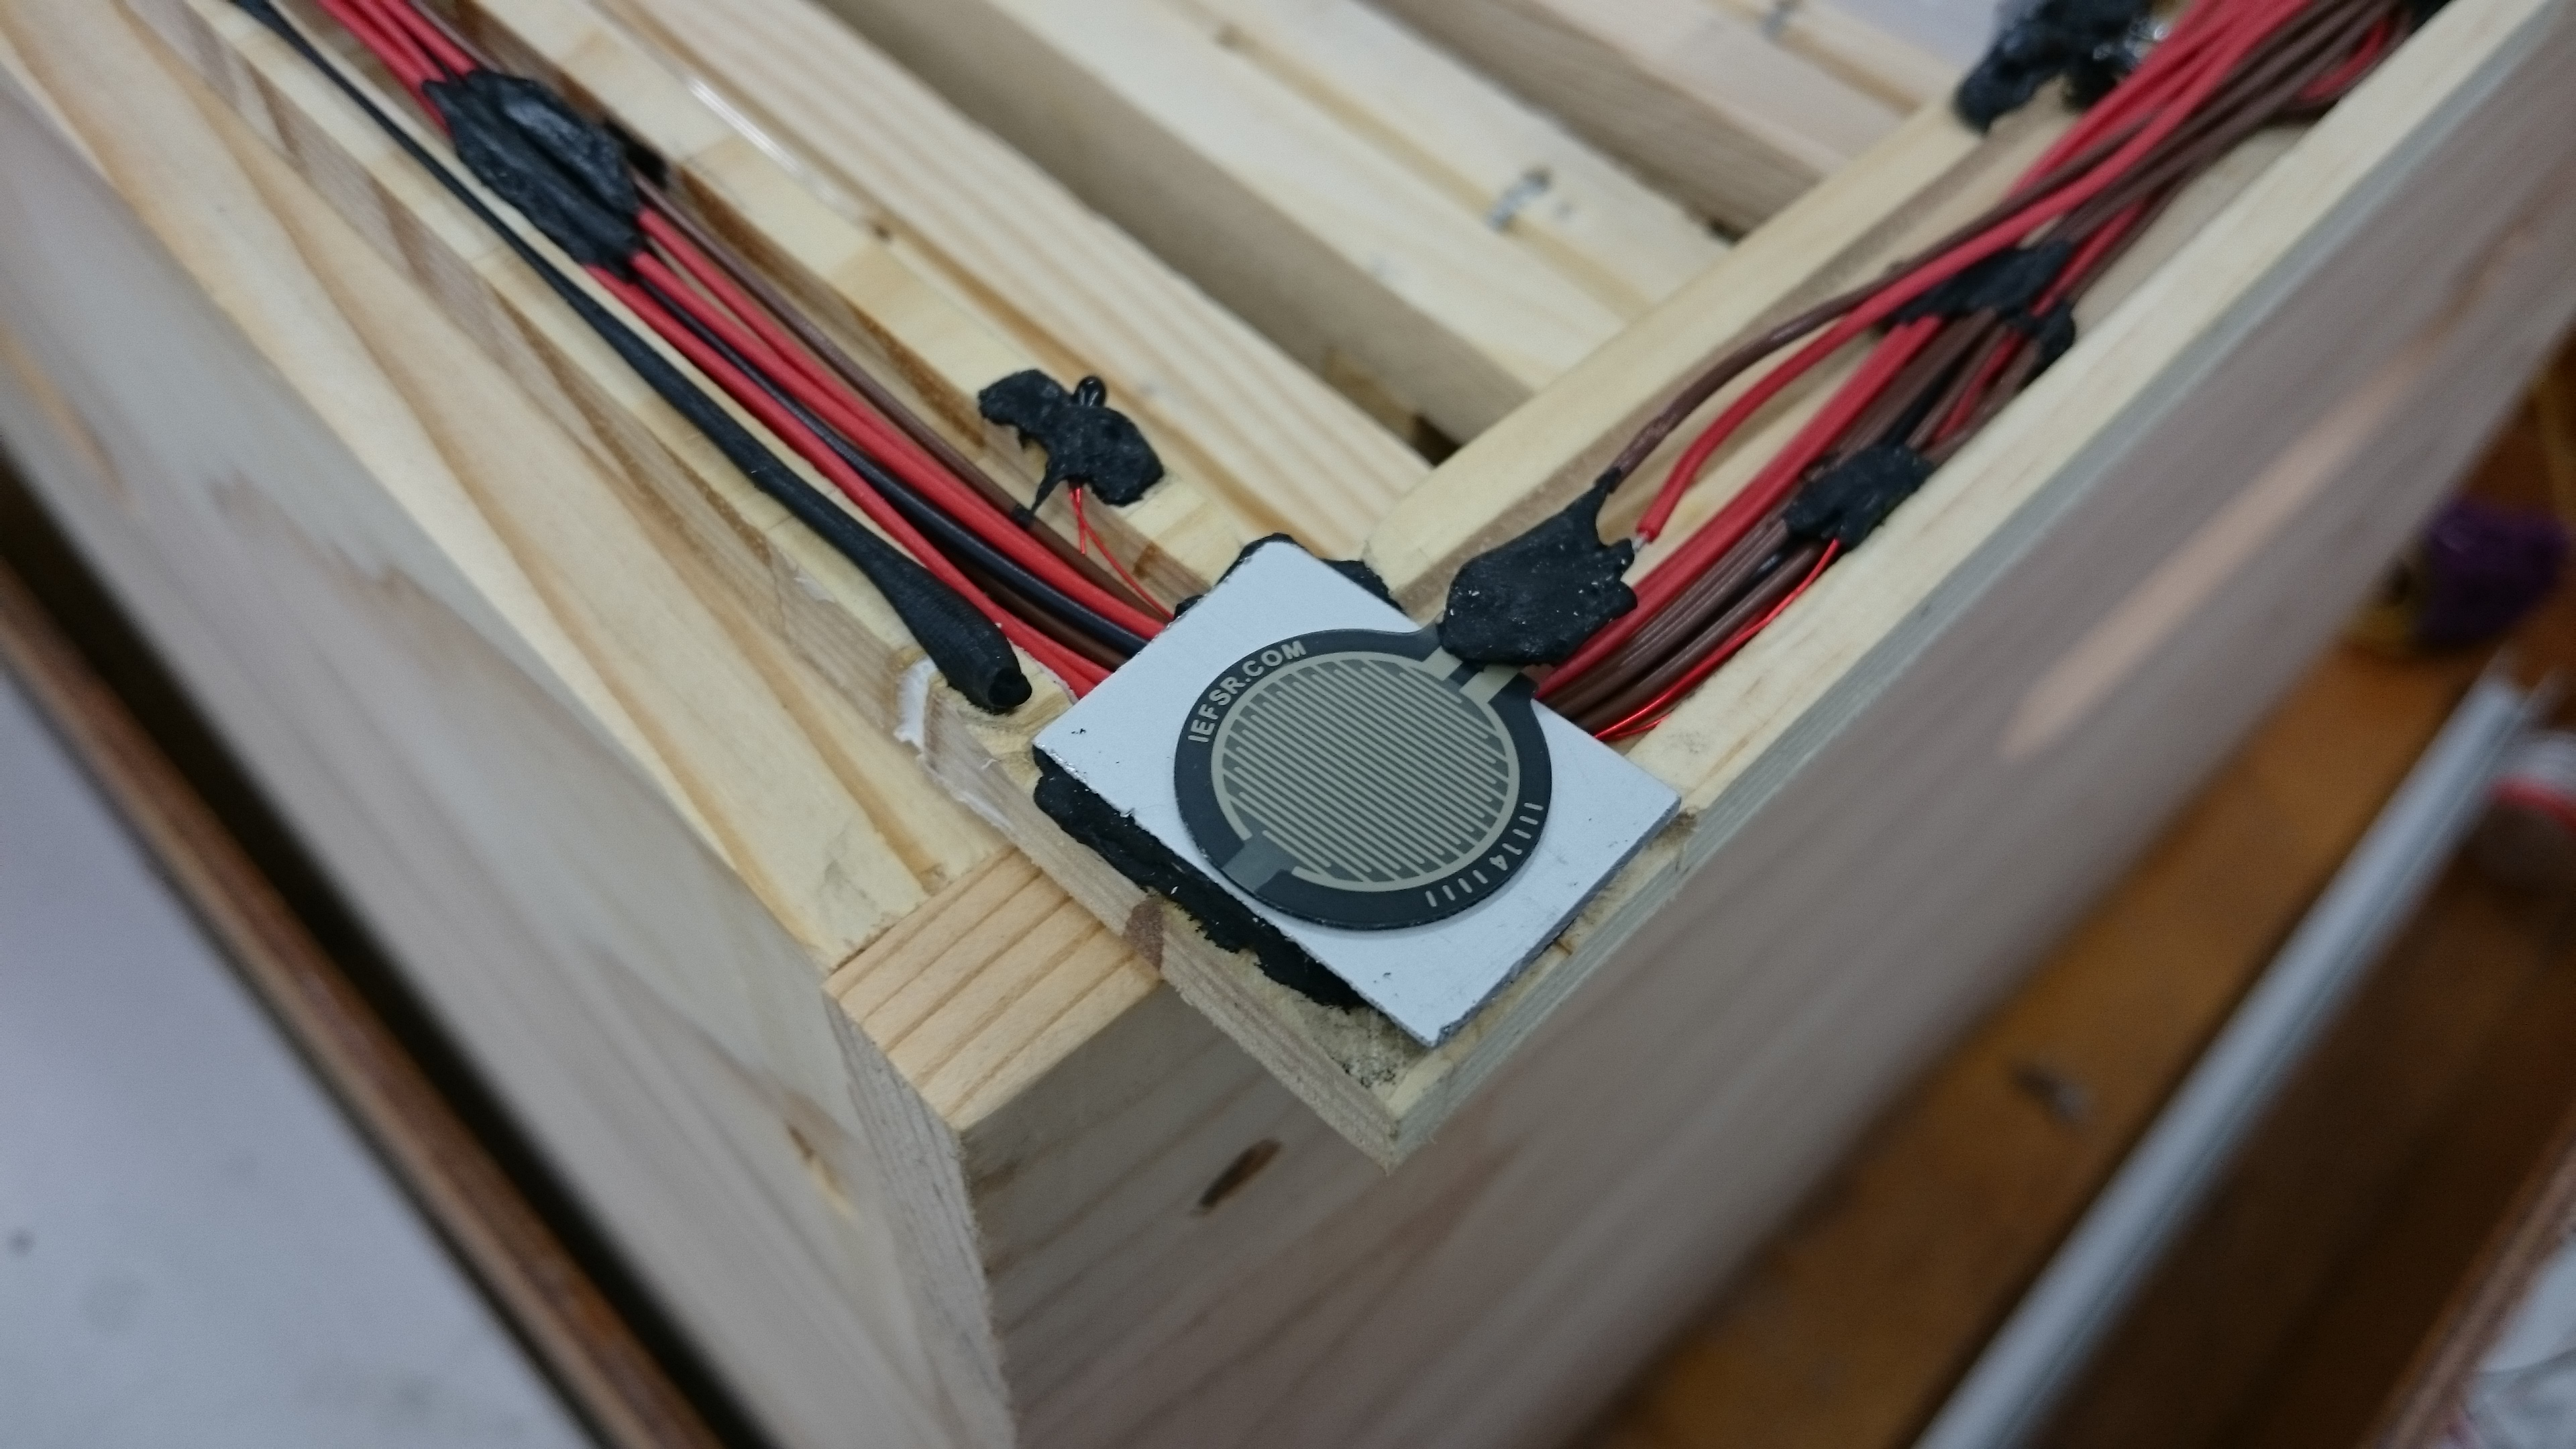
\includegraphics[trim= 0cm 0cm 0cm 0cm,scale=0.08]{pression.jpg}
\caption{\label{fig:pression2} Capteur de pression en position}
\end{figure}

Après avoir installé 2 tilt afin de recueillir le déplacement de la ruche dans 2 directions orthogonales et l'ensemble des autres capteurs (voir figure \ref{fig:cadre2}), nous avons recouvert le cadre avec 4 plaques en métal augmentant ainsi la rigidité. L'isolation a été réalisé grâce à l'emploi d'un mastique placé entre le bois et le métal ainsi qu'à l'intérieur du cadre pour maintenir les fils en place. \\
Une gaine en plastique sera placée à la sortie du cadre pour préserver l'isolation et permettre aux fils de rejoindre la carte où se situent la plaque sur laquelle les 6 thermistances et les 4 capteurs de pression sont placés. Cette plaque, la carte Arduino MEGA 2560, le module GSM/3G de Cooking Hacks et l'antenne seront placés dans un boitier à proximité de la ruche.     

\begin{figure}[h!]
\centering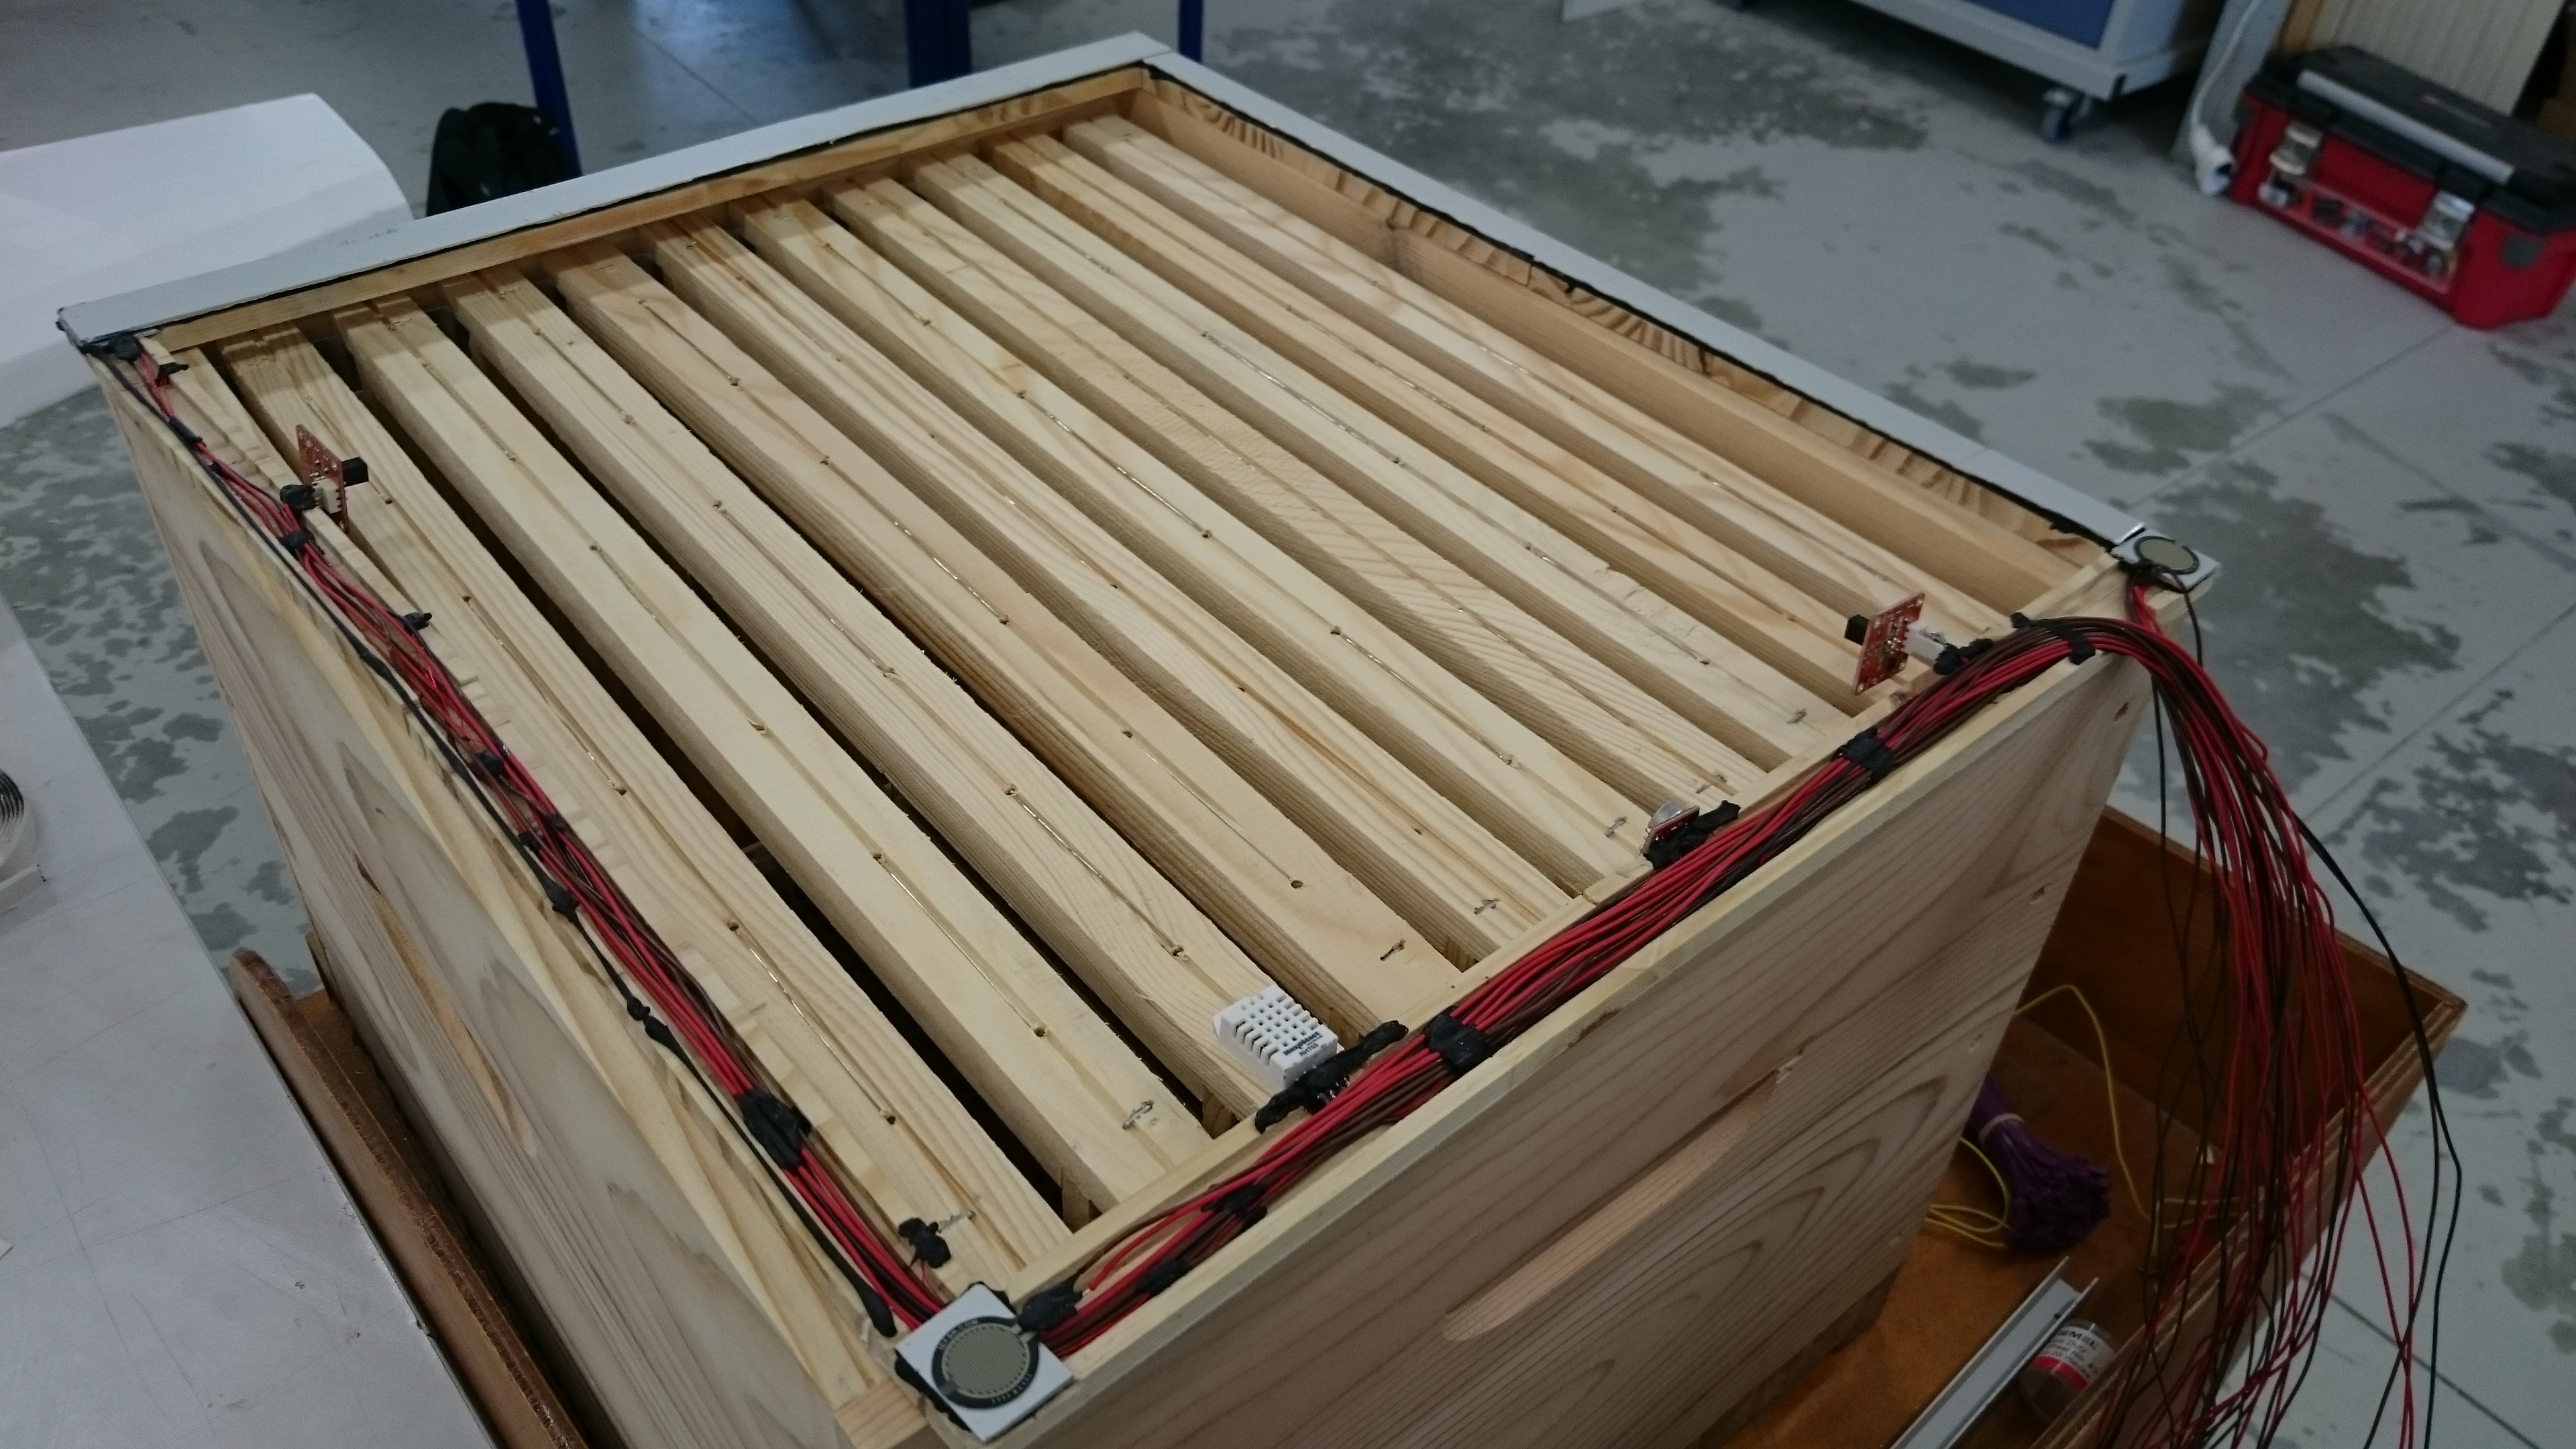
\includegraphics[trim= 0cm 0cm 0cm 0cm,scale=0.08]{cadre2.jpg}
\caption{\label{fig:cadre2} Cadre en cours de montage}
\end{figure}

\clearpage

\section{Gestion des données par Arduino}

Une fois les données recueillis par les capteurs et envoyées vers la carte Arduino, les deux principaux objectifs sont de pouvoir les stocker en local sur une carte SD et de pouvoir les envoyer au serveur pour que l'apiculteur puisse les consulter quelque soit sa position. Pour se faire, nous utiliserons le module GSM/3G de Cooking Hacks de la figure \ref{fig:shield}. Après avoir contacté un grand nombre d'opérateurs téléphonique sur Brest et n'ayant pu obtenir de une carte SIM pour notre projet, nous avons décidé d'utiliser nos propres cartes. 
Le module se programme à l'aide de commande AT (ATtention) qu'il faut exécuter dans un certain ordre en fonction de l'action désirée: envoyer un sms (AT+CPIN=****), établir une connexion HTTP (AT+CHTTPACT=url,port où le port est égal à 80 pour le protocole HTTP)...\\ 
Ces commandes sont spécifique au module que nous utilisons. Dans notre cas, il s'agit d'un SIM 5218 présent sur la figure \ref{shield}.

\begin{figure}[h!]
\centering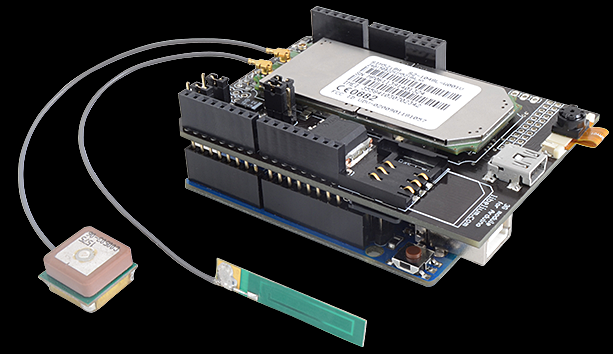
\includegraphics[trim= 0cm 0cm 0cm 0cm,scale=0.50]{shield.png}
\caption{\label{fig:shield} Shield GSM/3G connecté avec une Arduino UNO avec l'antenne de communication et GPS}
\end{figure}

Afin de tester progressivement notre code et comprendre la source des erreurs, nous avons utilisé une carte Arduino UNO en mode Gateway (en retirant le microcontrôleur ATmega) puis en rentrant les commandes AT via le monitor. En effet, il est impossible de retirer me microcontrôleur d'une Arduino MEGA 2560 l'endommager. Le monitor doit être réglé en mode CR-LF (Carriage Return - Line Feed) et choisir une vitesse de transmission de 115200 bauds. Il faut aussi veiller à placer les "jumpers" en position USB et non plus Arduino. Il nous a ensuite fallu télécharger la bibliothèque Time qui permet d'horodater nos mesures lors de leur enregistrement sur la carte SD et pour pouvoir satisfaire le format JSON utilisé par la base de données du serveur.

\clearpage

\begin{figure}[h!]
\centering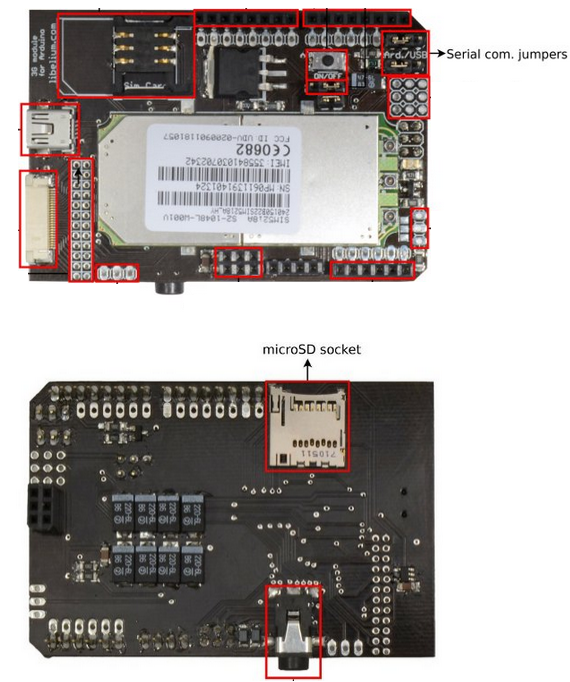
\includegraphics[trim= 0cm 0cm 0cm 0cm,scale=0.50]{jumpers.png}
\caption{\label{fig:jumpers} Vue détaillée du module GSM/3G et de la carte SIM 5218}
\end{figure}

Lorsque nous ne sommes plus en mode Gateway, il faut bien veiller à vérifier/téléverser notre code Arduino avant de connecter le shield GSM/3G. \\
Pour établir une connexion HTTP avec notre module GSM/3G, nous avons utilisé le site http://requestb.in qui permet de créer une URL temporaire que l'on peut utiliser pour effectuer des requêtes GET/POST. On peut alors voir sur ce site si ces requêtes ont bien été reçues. \\
L'alimentation de la carte Arduino sera assurée par des piles. 

\begin{figure}[h!]
\centering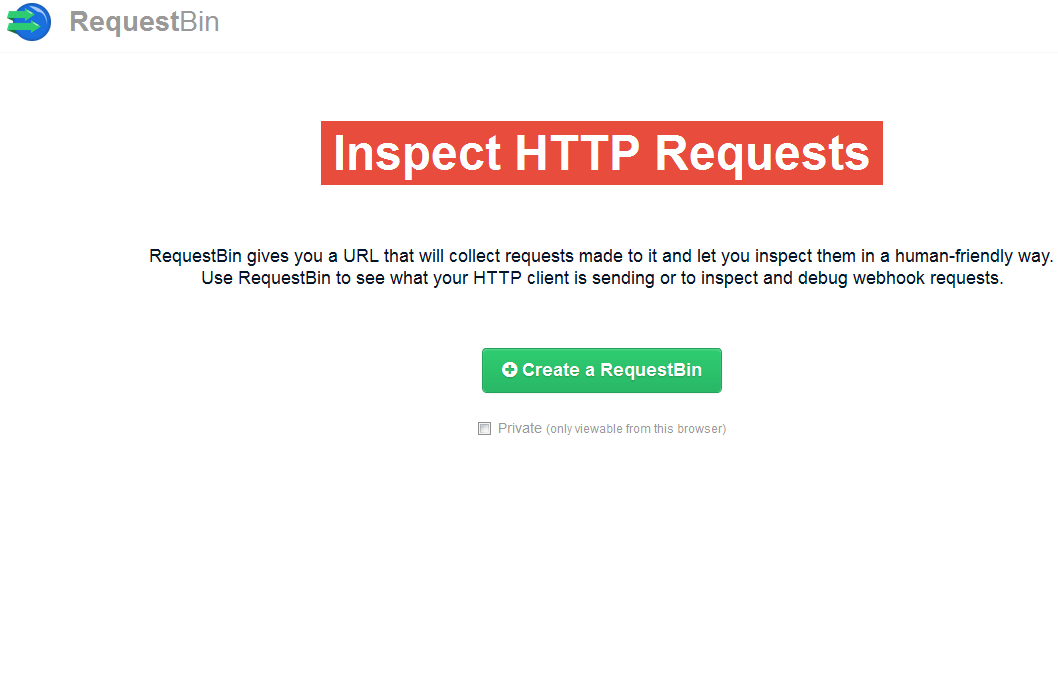
\includegraphics[trim= 0cm 0cm 0cm 0cm,scale=0.45]{requestBin.png}
\caption{\label{fig:requestBin} requestBin}
\end{figure}
\chapter{Server}
\section{Virtual Machine}

During the development of the BMONS systems, we opted for the utilization of a Virtual Machine. A virtual machine is a way to emulate a particular computer system from another system. Considering that most of the development would take place during class and inside the school's labs, we are faced with one issue: not having full administrator powers and full control of the software we are allowed to install. Having a complete virtual machine also allows a full portability of our development environment since it's common that the actual physical machines used for development vary between classes. Another advantage includes reducing the stress of deployment and developing in a safe environment. Once the project is done, it is possible to just copy the virtual machine to its final destination instead of doing a full reinstall of the system. Should any problems occur during the development, like corruption of the essential packages, for example, it will not affect the main system from which the virtual machine is loaded. Multiple virtual machines can co-exist in a hard drive, each one having its own full environment, using different softwares installed and eliminating possible conflicts. Even though a virtual is somewhat "closed", it is possible to share files between the main system (host) and a virtual machine (guest) using specific partitions. 

By using the software called Oracle VM VirtualBox, we were able to create a full development environment in a virtual machine with the Ubuntu operational system version 14.04. Ubuntu was our choice of operational system because it combines the power and possibilities of a Unix system, useful packages installed out of the box and a friendly Graphical User Interface. All that while still being completely free to use, since Ubuntu is an open source software. 

Once the operational system is installed on the virtual machine, it might be necessary to configure a network proxy so it is possible to access the internet from within. That is the case when using computers from the school's labs. Using Ubuntu, however, this is not such a difficult task. A proxy can be added by accessing System's Settings > Network > Proxy. 

\clearpage
\begin{figure}[h]
\centering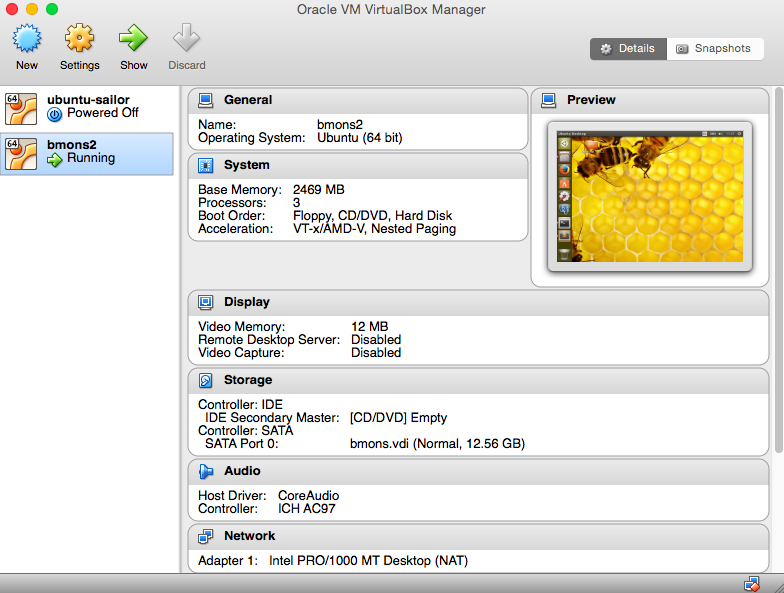
\includegraphics[scale=0.5]{virtualbox.png}
\caption{\label{fig:virtualbox} Oracle VM VirtualBox Software}
\end{figure}

\begin{figure}[h]
\centering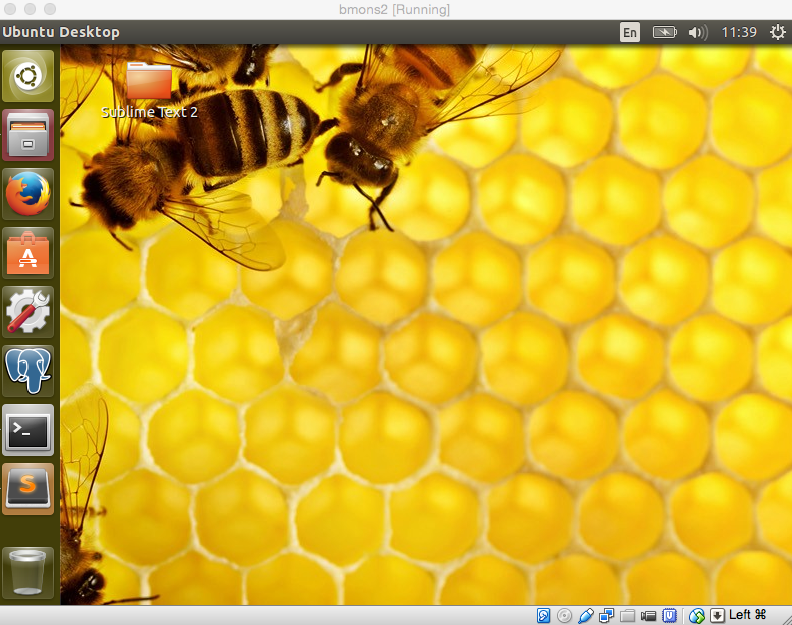
\includegraphics[scale=0.5]{ubuntu.png}
\caption{\label{fig:ubuntu} Ubuntu 14.04 loaded from Oracle VM Virtual Box}
\end{figure}

\clearpage

\section{Basic packages and installation}

To install BMONS on the virtual machine, it is firstly necessary either to download BMONS from the github repository located at https://github.com/Etiene/sailor/archive/master.zip or to download at least the file called install.sh, located at the directory /scripts/server.

Even though a virtual machine allows a portable environment, eliminating the need to install all software needed everytime a developer changes computers, sometimes errors might occur and a fresh install of the system might be necessary. This is why BMONS is provided with a install script for the server side. A bash script, extension .sh, runs multiple commands that normally would be necessary to be ran in the command line terminal and is very useful for automating tasks or a repeated sequence of commands. The install.sh file provided with BMONS will, then, automatically install most of the required software to run the BMONS server and modify it. Please note that this script should be run by the root user or using the privileges of the root user by using sudo.

\indent cd <location of BMONS at the filesystem>/scripts/server
\indent sudo ./install.sh

Among the essential packages installed by this script you will find: Git, the version control software used to keep track of BMONS; Ruby, the server-side programming language used on BMONS's website; Rails - the framework over which BMONS's website is developed; PostgreSQL - the database used to store BMONS's data; and pgAdmin III - a GUI (Graphical User Interface) software to administrate PostgreSQL.

An IDE (Integrated Development Environment) is not provided with the install script. Not only some IDEs are needlessly heavy, we believe that each developer has the right to choose their preferred way to write their code. The choice of our team was to use regular text editors, like gedit or Sublime Text (recommended).

\clearpage
\section{Webserver}

BMONS's website's server files are located under the directory bmons-site of our files. 

Before the first use of BMONS, it is necessary to navigate to this directory and run 'bundle install' and 'rake db:schema:load' at the command line. Please note that this step is not necessary if you are running BMONS from a previously configured virtual machine. This is required only if it is a fresh install of BMONS and only before the first time of running the webserver.

\indent cd <location of BMONS at the filesystem>/bmons-site
\indent bundle install
\indent rake db:schema:load

BMON's website uses some third-party softwares that made the development phase more productive, such as Devise, for example. Devise is a full-featured authentication solution which handles all of the controller logic and form views. This was used to implement the login system for BMONS. Running 'bundle install' will install all the necessary gems (plugins for the Ruby language) required to run Rails and the other gems that we chose to use during development. 

When installing the server for the first time, the database will be empty. It will not contain the tables that store our data. This is why the command 'rake db:schema:load' is necessary. It will load the schema of the entities used by the website and generate the queries that will create those tables.

To start the server, it is necessary to run the command 'rails server'.

\indent cd <location of BMONS at the filesystem>/bmons-site
\indent rails server

Once that is done, the website will be accessible via the url configured.

\clearpage
\section{Database and Backup}

The choice of database our team made for BMONS was PostgreSQL. Many options were possible but there are some advantages to using this specific one. While NoSQL databases are interesting and can be very fast in terms of performance, they are not very easy to deal in terms of development. Also, NoSQL is usually very fast for accessing and reading data but not so fast for writing and inserting data. Normally, BMONS should insert data way more frequently than reading. That is because one single user that is not connected to the website the whole time can have multiple beehives that will be sending data to the server on a regular basis, making us to reject this option right away. In addition to this, the archirecture of BMONS's data is already compatible with a regular SQL relational data.

There are many possible options of SQL databases, however, among those, PostgreSQL was favored because our team already had some knowledge of it and because it is a very good, reliable and stable open source software that is capable of dealing with very high volumes of data if necessary.

It is recommended to do database backups regularly. In case data is corrupted, it will be possible to restore the original data from recent a backup. BMONS is provided with a script that will automatically dump the database data into a dated file in the filesystem regularly (every 3 hours). It is recommended that that these generated files are copied to a safe location, such as another computer or an external hard drive from time to time.

Cron is an automatic scheduler for Unix systems that will run command line commands in specific times or time intervals according to the following pattern:
  #comment
  * * * * *  command to execute
  │ │ │ │ │
  │ │ │ │ │
  │ │ │ │ └───── day of week (0 - 6)
  │ │ │ └────────── month (1 - 12)
  │ │ └─────────────── day of month (1 - 31)
  │ └──────────────────── hour (0 - 23)
  └───────────────────────── min (0 - 59)

To activate the automatic backups, it is necessary to navigate to the directory /scripts/server of BMONS files. Under this directory is located a file called cron.txt. When making a fresh install of BMONS, it might be necessary to edit the line 6 of this file and correct the path to the backup bash script. It is also possible to change the frequency of the backups if desired. 
 
\texttt{0 */3 * * * /home/bmons/BMONS/scripts/server/db\_backup.sh}

Then you can run the following command to incorporate this cron job into the schedule:

\indent crontab cron.txt

\clearpage
\section{The web interface}

The web interface of BMONS was built using Ruby on Rails. Rails is an open source web application development framework written in the Ruby language. It's used specially for developing database-driven websites and allows the creation of applications using pre defined structures. Rails is a Model-View-Controller (MVC) framework. MVC is a software design pattern for implementing user interfaces. It divides the software into three interconnected parts. 
Models: They store the data of the application, its business rules and methods. It's often regarded as a "mirror" of the database.
Views: They're the output of a model data representation, such as a table or a diagram, for the user.
Controllers: They make the mediation between the models and the views, sending commands to update models' states and sending commands to the view to alter the presentation of the models.

The Rails philosophy includes two major guiding principles:

"Don't Repeat Yourself: DRY is a principle of software development which states that "Every piece of knowledge must have a single, unambiguous, authoritative representation within a system." By not writing the same information over and over again, our code is more maintainable, more extensible, and less buggy.
Convention Over Configuration: Rails has opinions about the best way to do many things in a web application, and defaults to this set of conventions, rather than require that you specify every minutiae through endless configuration files."

Rails philosophy and features allowed our team to develop an interesting application in a feasible time. This web application allows a beekeeper to register, login, change password, see a dashboard with visual data from their hives and manage hives and alerts. The application will also receive content from the Arduino located at the hive and update its data.

The authentication system was developed with the use of Devise, which is a plugin that fully handles the authentication through the MVC pattern. The pages to manage beehives, sensors, measurements, alerts and alert logs were firstly created with the use of scaffolding. A scaffold in Rails is a full set of model, database migration for that model, controller to manipulate it, views to view and manipulate the data, and a test suite for each of the above. This scaffold can be created through the command line in a very easy manner.

rails generate scaffold Beehive name:string user:references position:string mode:string

However, scaffolding alone is not enough and after the creation it is necessary to rearrange and modify the code to make it suit our needs. One example is modifying the beehive scaffold for showing only the beehives that belong to the user currently logged in.

One important aspect of the BMONS's website is the design. The design was developed with the help of Bootstrap. Bootstrap is a free and open source front-end framework that uses HTML, CSS, and JavaScript to provide re-usable components and other interface elements. It allows the development of responsive and mobile first projects on the web. With some customization Bootstrap, we were able to obtain pages that display our system's contents beautifully. We opted for changing the color palette into a yellow
and dark gray theme on a light background because it's aesthetically beautiful, readable and refers well to a bee's color pattern.

Bootstrap, however, is not enough for displaying our data. The dashboard requires the data to be easily grasped and even though tables are really useful, they are not sufficient to provide a quick visual analysis. Our team's choice of optimal display was a graphical one. The development of the graphical dashboard was made with NVD3, a JavaScript library that extends another library called D3 that allows you to bind arbitrary data to a Document Object Model (DOM), and then apply data-driven transformations to the document. The advantage of using NVD3 over D3 is that it is an easier to use library with a reduced collection of components that satisfies our needs without taking away the power of D3. The data is then passed from the controller backend in ruby to the frontend view in a JavaScript piece of code that is then used and manipulated by the NVD3 library, producing beautiful results. The graphic allows for the visualization of measures from sensors in time of each individual beehive, allowing to switch between hives without refreshing the page. 

\clearpage
\begin{figure}[h]
\centering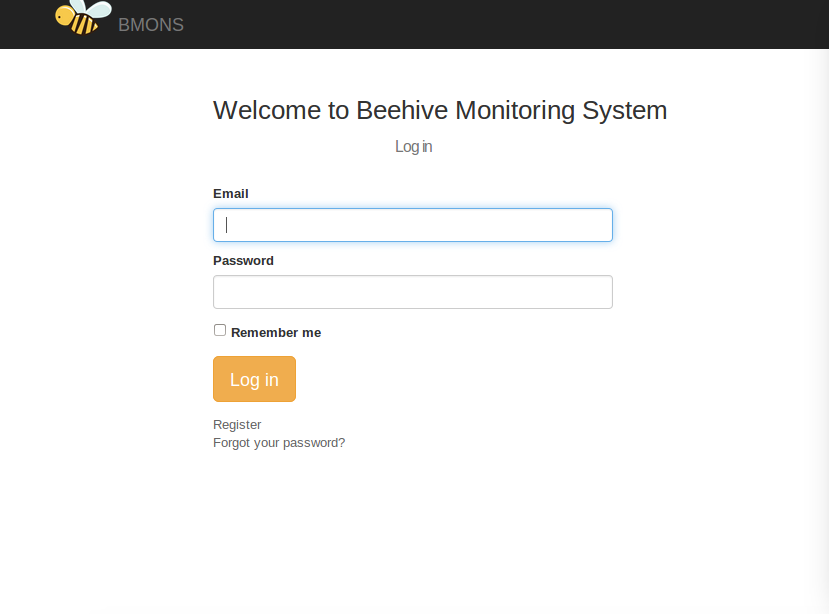
\includegraphics[scale=0.5]{login.png}
\caption{\label{fig:login} Initial page of BMONS web page. User authentication is necessary. }
\end{figure}

\begin{figure}[h]
\centering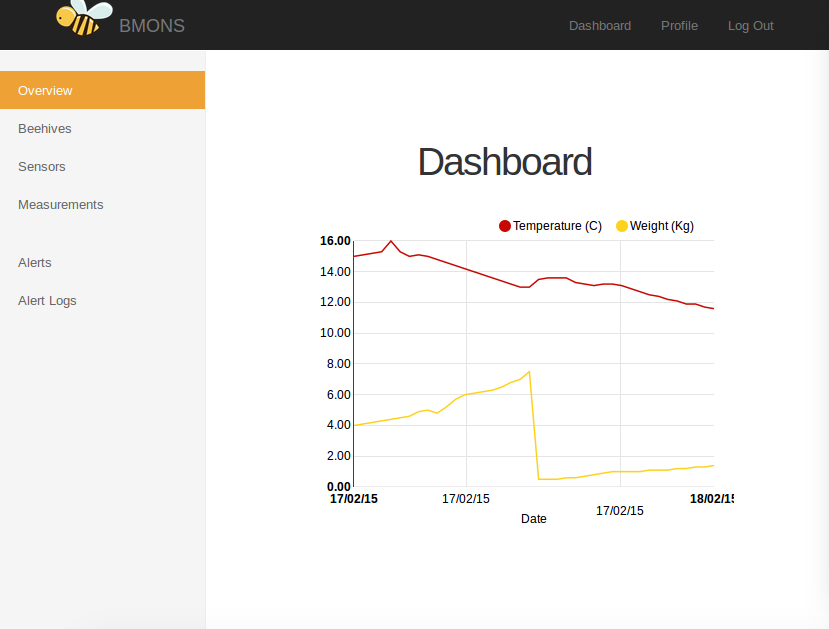
\includegraphics[scale=0.5]{dashboard.png}
\caption{\label{fig:dashboard} The initial page once the user is logged in shows the dashboard. }
\end{figure}

\begin{figure}[h]
\centering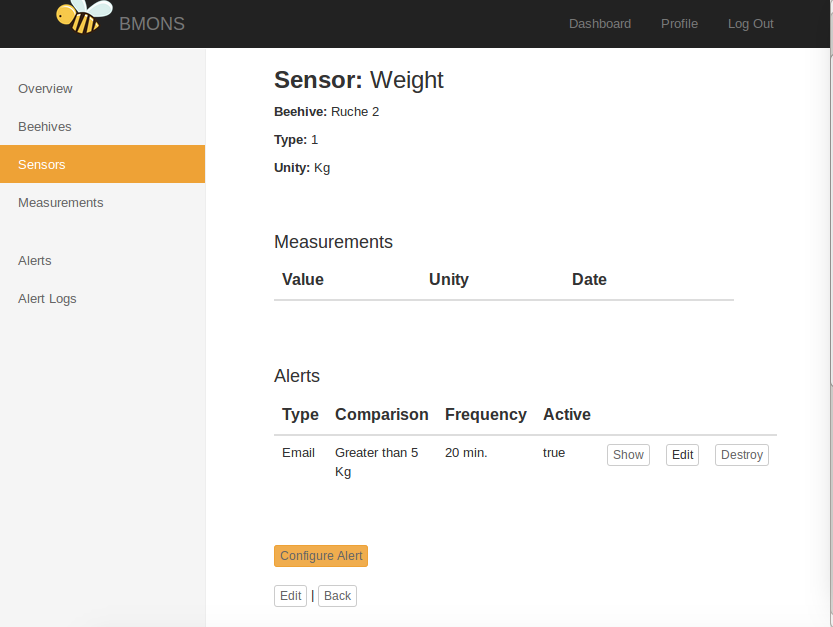
\includegraphics[scale=0.5]{sensor.png}
\caption{\label{fig:sensor} Page that shows a sensor information }
\end{figure}

\begin{figure}[h]
\centering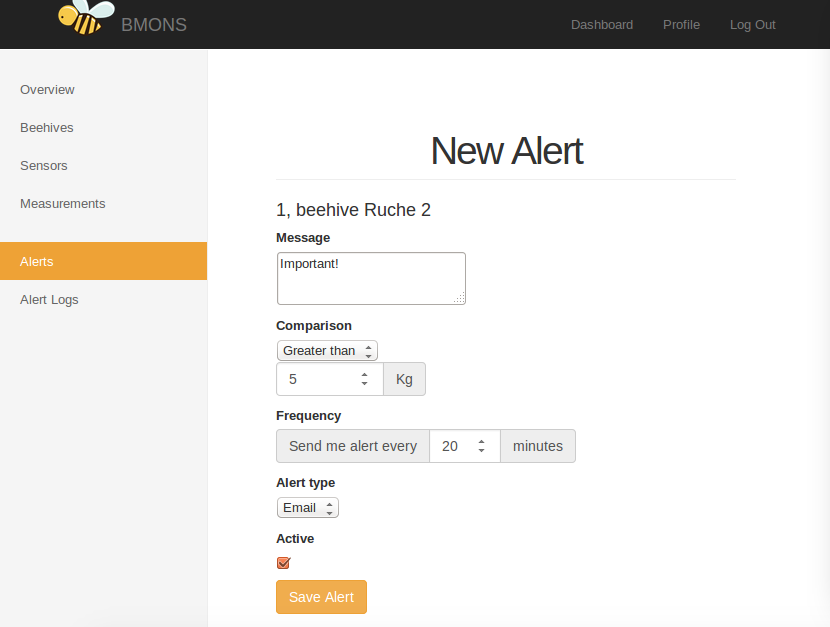
\includegraphics[scale=0.5]{alert.png}
\caption{\label{fig:alert} Page to create a new alert. }
\end{figure}

\clearpage

\section{The API and receipt of data from external source}

BMONS contains an API for receiving the captured data by the Arduino and storing it on a database for later displaying to the beekeeper. By default a Ruby on Rails CRUD (create, read, update and delete actions for an entity) is already a REST (Representational State Transfer) API that will perform the necessary actions using the right HTTP protocol request method and with full JSON capability. A PATCH or PUT will access the update action, a GET will obtain the data in a JSON object as a response, a DELETE will access the delete action and destroy the desired data and, finally, a POST will receive a JSON object and store new data. For BMONS needs, it was necessary to use the POST request to receive new measurements periodically from an external source, the Arduino, instead of from a form in a view used by an authenticated user. To make sure the data coming in is still safe, for the measurement create action, instead of a user authentication, a Basic HTTP Authentication is used. That means that the POST request sent by the Arduino must also send an authentication token on its header and the data will only be stored if the details are correct. In addition to the authentication, the Arduino must also sent, of course, the data. The content-type of this request should be application/JSON and a JSON object containing the necessary information for creating a new measurement should be included in the body of the request. To test BMONS's RESTful API, a browser extension named Postman was used as a client. 

\input{BilanVFU}

%----------------------------------------------------------------------------------------
%	PART V 
%----------------------------------------------------------------------------------------
\part{Perspectives d'amélioration}
\chapter{La collecte et la transmission de données}

\section{Communication Wifi}

Un des points qui peu être amélioré dans notre projet est le système de transmission de données. Nous avions opté pour une transmission GSM/3G en supposant que la localisation des ruchers ne pouvaient pas être couverte par un réseau Wifi. Cela obligera donc l'apiculteur à se procurer une carte SIM chez un opérateur téléphonique. Or, ce mode peut devenir couteux sur plusieurs de ses ruches sont équipés de notre cadre. C'est pour cela qu'il peut être intéressant de développer un système de communication Wifi en plus de celle GSM/3G en fonction du lieu des ruches. Nous avons commencé à développer ce type de transmission avec les modules Wifi présents au club robotique de l'ENSTA Bretagne en se reposant sur le protocole HTTP.   

\begin{figure}[h!]
\centering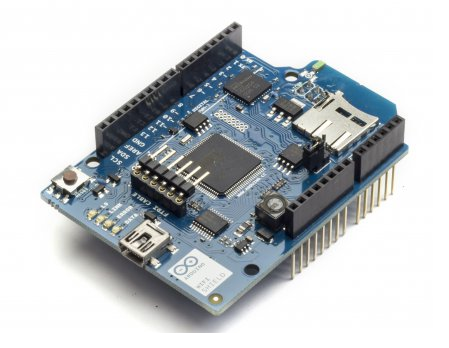
\includegraphics[trim= 0cm 0cm 0cm 0cm,scale=0.65]{wifi.png}
\caption{\label{fig:wifi} Shield Wifi Arduino}
\end{figure}

\clearpage

\section{Traitement du son}

Le cadre de mesure possède bien un capteur de son permettant de recueillir le bruit ambiant et renseigner l'apiculteur sur la présence d'abeilles et l'activité de sa ruche. Néanmoins, l'état de l'art mené nous a permis de connaitre la fréquence émise par les ouvrières avant un essaimage. L'idée est de pouvoir effectuer un traitement du signal sonore reçu et repérer la fréquence d'essaimage. Nous avons essayer de repérer des fréquences "pures" générées en utilisant Audacity et Matlab pour tester les capacités de notre capteur avec succès bien malgré un bruit important.
Pour cela, deux solutions sont envisageables: \\

\indent - Télécharger la bibliothèque FFT d'Arduino présente sur GitHub. \\
\indent - Prévoir un programme de traitement du son sur le serveur. \\

Dans les deux cas, nous avons aussi envisagé un filtre physique placé à la sortie du capteur de son afin d'avoir un meilleur filtrage en amont.

\begin{figure}[h!]
\centering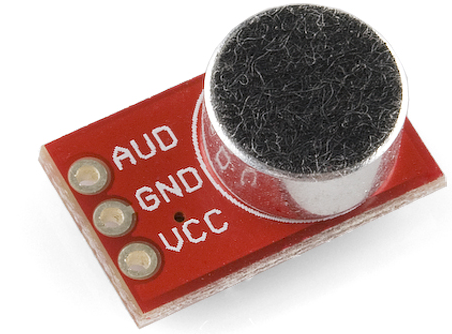
\includegraphics[trim= 0cm 0cm 0cm 0cm,scale=0.5]{son.png}
\caption{\label{fig:son} Capteur de son présent dans le cadre de mesure}
\end{figure}

\section{Alimentation}

Pour l'alimentation, il peut être intéressant de développer un système informant l'apiculteur de l'état des piles/batteries présents dans le boitier avec la carte Arduino. \\
Il pourra aussi être intéressant de développer un système plus écologique comme par exemple une éolienne ou des panneaux solaires que nous disposerons au milieux du rucher et où les différents cadres viendront s'alimenter. Coupler cette solution avec une communication Wifi permettra à l'apiculteur d'utiliser le système de cadre de mesure pour un coup minimal. 

\section{Server}

For the moment, for each new measurement a POST request needs to be made. In the case there are many users with many beehives, there will be many requests being made and that could cause a strain on the server, having an impact on scalability. In the future, it should be possible to send new measurements in batches, one single POST request would send a JSON object containing the values for all sensors to that Arduino. It would also be interesting to create a queue. If there is a connectivity problem, the data will wait and then be sent in a single request once connectivity is restored, causing the data not to have "holes" in its timeline.

Another possible improvement is, when creating a new beehive at the web application, it would already create a set of basic sensors that are most commonly used. This would allow a quicker configuration for a new beekeeper's account. 

It would also be optional if the web application generated a text file that could be incorporated into the Arduino, and the Arduino would read from that file and understand which physical sensor corresponds to which unique database entry, automating a configuration that is, for the moment, manual. 
\chapter{Conclusion}\\
Le projet BMONS a pour ambition de réaliser un système embarqué sur une ruche pour récolter les paramètres physiques de la ruche dans l’optique de détecter les anomalies de comportement des abeilles. Notre équipe s’est donc penché sur cette problématique avec des notions d’apiculture et de conduite de projet plutôt minces.

Après la première partie du projet nous pouvons enfin dire que nous comprenons les besoins et les attentes des apiculteurs, par exemple des fonctions auxquelles nous avions pensé, comme la détection du taux d'humidité dans la ruche ne semblent finalement pas primordiale au projet. En revanche des options comme le comptage des abeilles seraient appréciées par les apiculteurs, mais des compromis doivent êtres faits car certaines de ces options entrainent un surcoût trop conséquent pour que le projet satisfasse les exigences initiales.\newline 

Nous devons une grande partie de ces connaissances en apiculture aux réponses précises de monsieur Franck Singhoff, qui nous a également prêté une ruche pour que nous puissions travailler sur l'implémentation des capteurs sur notre prototype. \newline 

Les difficultés que nous avons rencontrées, par exemple lors de la compréhension et de la création des diagrammes nécessaires à l'établissement de la spécification fonctionnelle sur les trois axes, ont été surmontées grâce à l’aide de nos encadrants de projet, mais aussi grâce au dialogue entre les membres du groupe. Les choix des divers composants qui constitueront le prototype ont aussi été une source de problèmes, car même si nous avions une idée de quel type de composant nous avions besoin, faire le tri entre tous ceux qui existent nécessite de faire des choix entre par exemple le prix et la précision d’un capteur, et cela influe sur les exigences du projet. Enfin, la mise en place du serveur et de la création du cadre de mesure nous a permis d'acquérir des connaissances en protocole HTTP et en programmation Arduino. Nous avons pu ainsi être confronté aux problèmes de la communication sans fil.\newline

Ces quelques mois de travail en commun nous ont permis d'avoir un aperçu d'ensemble de la conduite d'un projet. Nous nous sommes rendu compte de la quantité de travail que représente la partie ingénierie système sur un projet comme celui-ci. Néanmoins, cette partie nous a permis de mieux anticiper l'intégration des capteurs et nous a donné une meilleure vision de la gestion de la base de données. 






\appendix
\part{Annexes}
 

\backmatter % Partie finale du document, non numérotée

%----------------------------------------------------------------------------------------
%	BIBLIOGRAPHIE
%----------------------------------------------------------------------------------------
%\addcontentsline{toc}{part}{Bibliographie}
%\bibliographystyle{apalike-fr}
%\bibliographystyle{plain-fr}
%\bibliography{bibliographie}
%\nocite{*}

%----------------------------------------------------------------------------------------
%	INDEX
%----------------------------------------------------------------------------------------
\cleardoublepage
\phantomsection
\setlength{\columnsep}{0.75cm}
\addcontentsline{toc}{part}{Index}
\label{sec:index}
\printindex

%----------------------------------------------------------------------------------------
%	GLOSSAIRE
%----------------------------------------------------------------------------------------
\cleardoublepage
\phantomsection
\setlength{\columnsep}{0.75cm}
\addcontentsline{toc}{part}{Glossaire}
\printglossaries

%----------------------------------------------------------------------------------------

\end{document}